\documentclass[11pt,a4paper]{article}

% ---------------------------------------------------------------- packages
\usepackage[T1]{fontenc}
\usepackage[utf8]{inputenc}
\usepackage{lmodern}
\usepackage{microtype}
\usepackage[margin=2.5cm]{geometry}
\usepackage{amsmath,amssymb,bm}
\usepackage{booktabs,tabularx,multirow,array}
\usepackage{graphicx}
\usepackage[font=small,labelfont=bf]{caption}
\usepackage{subcaption}
\usepackage{xcolor}
\usepackage{enumitem}
\usepackage[section]{placeins}
\usepackage{tikz}
\usetikzlibrary{arrows.meta,positioning,fit,backgrounds,calc,shapes.geometric}
\usepackage[numbers,sort&compress]{natbib}
\usepackage[colorlinks=true,linkcolor=blue!50!black,citecolor=green!40!black,urlcolor=blue!60!black]{hyperref}
\usepackage[nameinlink,capitalise]{cleveref}

\graphicspath{{../figures/}{../../results/}}
\setlist{itemsep=2pt,topsep=4pt}
\newcommand{\NDCG}{\mathrm{NDCG}}
\newcommand{\Hit}{\mathrm{Hit}}
\newcommand{\MRR}{\mathrm{MRR}}

\definecolor{cdata}{HTML}{E8EAED}
\definecolor{cllm}{HTML}{D2E3FC}
\definecolor{cdl}{HTML}{FCE8E6}
\definecolor{cbase}{HTML}{E6F4EA}
\definecolor{cfuse}{HTML}{FEF7E0}

\tikzset{
  box/.style={draw, rounded corners=3pt, align=center, minimum height=1.0cm, inner sep=4pt, font=\small},
  arr/.style={-{Stealth[length=2.2mm]}, thick},
  grp/.style={draw, dashed, rounded corners=6pt, inner sep=7pt},
}

% ---------------------------------------------------------------- title
\title{\textbf{Agentic LLM Ranking versus Trained Sequential Models:\\
An Audited Study of ARAG, GRU Fusion and Text-Aware Sequence Modelling\\
on Amazon Reviews 2023 (Video Games)}}
\author{%
  \textit{[Author Name]}\\
  \textit{[Course / Programme --- Deep Learning Project]}\\
  \textit{[Institution]}}
\date{October 2026}

\begin{document}
\maketitle

% ================================================================ abstract
\begin{abstract}
\noindent Large language models (LLMs) can rank recommendation candidates by reasoning over a
user's history in natural language. ARAG \citep{maragheh2025arag} organises this reasoning as a
pipeline of four cooperating agents. We implement an ARAG-style recommender on the Amazon
Reviews 2023 Video Games category \citep{hou2024bridging} and ask whether a \emph{trained}
deep-learning component --- a GRU sequential model \citep{hidasi2016session} --- improves it
when late-fused into the LLM ranking. To isolate ranking from retrieval, every system ranks the
same frozen 20-item candidate list per user (the held-out next item plus 19
popularity-matched negatives), and all contrasts are tested with a paired bootstrap.
With \texttt{gpt-4o-mini}, ARAG reaches NDCG@5 $=0.424$ on 100 test users and significantly
beats the paper's LLM baselines; the paper's NLI+CSA ablation also reproduces significantly.
However, properly trained sequential models --- a comparison the paper does not make --- are
more accurate: on the same users a GRU reaches $0.520$, SASRec \citep{kang2018self} $0.536$
(ARAG $-$ SASRec $=-0.112$, 95\% CI $[-0.213,-0.009]$), and on all 94{,}762 test users our
\emph{text-aware GRU}, whose item vectors add a projected frozen MiniLM embedding of the item's
metadata, is best with $0.530$. Fusing the GRU into ARAG significantly improves ARAG
(H1: $+0.098$, $[+0.013,+0.182]$) but not the GRU (H2: $+0.004$, n.s.). ARAG's distinctive
advantage is not accuracy but a much lower popularity bias and higher catalogue coverage. We
document two errors found during the project --- a degenerate candidate construction and a GRU
weight-initialisation bug --- each of which had reversed a headline conclusion, and we release
an audit pipeline that re-derives every reported number from raw predictions. All
post-correction experiments required zero new LLM calls.
\end{abstract}

\noindent\textbf{Keywords:} recommender systems; large language models; agentic retrieval-augmented
generation; sequential recommendation; GRU4Rec; late fusion; evaluation methodology.

\tableofcontents
\newpage

% ================================================================ 1 intro
\section{Introduction}
\label{sec:intro}

Sequential recommendation predicts the next item a user will interact with from the order of
their past interactions. For a decade the standard tools have been neural sequence models trained
on interaction logs, from recurrent networks such as GRU4Rec \citep{hidasi2016session} to
self-attentive models such as SASRec \citep{kang2018self}. Large language models offer a
different route: they can read item titles and descriptions, infer a user's intent in natural
language and rank candidates zero-shot \citep{hou2024llmrank}. Agentic pipelines push this
further by splitting the task into specialised LLM calls. ARAG \citep{maragheh2025arag} uses
a \emph{User Understanding Agent}, a \emph{Natural Language Inference} agent, a \emph{Context
Summary Agent} and an \emph{Item Ranker Agent}, and reports large gains over single-prompt LLM
baselines.

The two families have complementary strengths. Trained models capture collaborative
co-occurrence patterns across hundreds of thousands of users, but see only opaque item IDs; LLMs
understand item content but see only one user at a time and cost several API calls per
recommendation. This project asks whether combining them helps, and what each contributes.

\paragraph{Research questions.}
\begin{description}[leftmargin=1.2cm,style=nextline]
  \item[RQ1] On identical frozen candidate lists, does late-fusing a trained GRU into ARAG's
  ranking improve over ARAG alone (\textbf{H1}) and over the GRU alone (\textbf{H2})?
  \item[RQ2] Do the base paper's claims --- ARAG beats simpler LLM baselines, and each agent
  component contributes --- hold on a new category and model?
  \item[RQ3] How accurate are trained sequential models (GRU, SASRec, and a text-aware GRU) on the
  same protocol, and how do they differ from ARAG beyond accuracy?
\end{description}

\paragraph{Contributions.}
\begin{enumerate}
  \item An ARAG-style four-agent recommender with strict JSON-schema outputs, a repairing
  ranking parser, and a disk cache that makes every LLM run exactly replayable at zero cost.
  \item A ranking-isolating evaluation protocol: frozen 20-item lists with popularity-matched
  negatives, a single shared user sample for all systems, validation-only tuning and paired
  bootstrap confidence intervals.
  \item For RQ1, fusion significantly improves ARAG (H1) but not the GRU (H2); for RQ2, a
  statistically significant reproduction of the base paper's baseline ordering and NLI+CSA
  ablation.
  \item Strong trained baselines the paper omits: GRU4Rec, SASRec and a \emph{text-aware GRU} that
  adds frozen sentence embeddings of item metadata to the item representation. All three are more
  accurate than ARAG at zero per-request cost; ARAG has far lower popularity bias (RQ3).
  \item Two documented methodological lessons: a candidate-list construction that let
  popularity-like systems win, and an embedding-initialisation bug that crippled the GRU. Each
  reversed a headline conclusion; we report the diagnosis, the fix and both sets of numbers.
\end{enumerate}

The rest of the report is organised as follows. \Cref{sec:related} reviews related work,
\cref{sec:data} describes the data and \cref{sec:protocol} the evaluation protocol.
\Cref{sec:method} presents the systems, \cref{sec:setup} the experimental setup and
\cref{sec:results} the results. \Cref{sec:discussion} discusses them,
\cref{sec:threats} lists threats to validity and \cref{sec:conclusion} concludes.

% ================================================================ 2 related
\section{Related Work}
\label{sec:related}

\paragraph{Sequential recommendation.} GRU4Rec \citep{hidasi2016session} introduced recurrent
networks \citep{cho2014learning} for session-based recommendation, trained with a next-item
objective. SASRec \citep{kang2018self} replaced recurrence with causal self-attention and is
today a standard strong baseline. Both models represent items by learned ID embeddings, so items
with few interactions receive poorly trained vectors --- a weakness that becomes acute when user
histories are short.

\paragraph{Text-based and transferable sequence models.} Several works replace or augment ID
embeddings with representations of item text. UniSRec \citep{hou2022unisrec} learns universal
item representations from text with a pre-trained language model so that sequence models
transfer across domains. Our text-aware GRU follows the same principle in its simplest form: a
frozen sentence encoder \citep{reimers2019sentence,wang2020minilm} supplies item features that a
learned linear projection maps into the GRU's embedding space, added to the ID embedding.

\paragraph{LLMs as recommenders.} LLMs can act as zero-shot rankers when given a user's history
and a candidate list in the prompt \citep{hou2024llmrank}. Retrieval-augmented variants select
which parts of the history to show. ARAG \citep{maragheh2025arag} decomposes ranking into
user understanding, candidate--user natural language inference, context summarisation and final
ranking, and reports gains of 25--42\% NDCG@5 over recency-based and vanilla RAG prompting on
three Amazon categories.

\paragraph{Evaluation methodology.} Sampled-candidate evaluation is cheap but can distort
system rankings, depending on how the negatives are drawn \citep{krichene2020sampled}. Strong,
well-tuned simple baselines often match complex neural recommenders
\citep{dacrema2019really}, which motivates our inclusion of content-similarity and
item-based collaborative filtering \citep{sarwar2001item} baselines. We use the paired bootstrap
\citep{efron1993bootstrap} for significance, with NDCG \citep{jarvelin2002cumulated} as the
primary metric.

% ================================================================ 3 data
\section{Data}
\label{sec:data}

We use the Amazon Reviews 2023 corpus \citep{hou2024bridging}, Video Games category, in its
official rating-only 5-core leave-last-out benchmark split. For each user, the last interaction
is the test target, the second-to-last is the validation target and the remainder is training
history. Each interaction is a user reviewing an item, the standard stand-in for a purchase
in this corpus (purchase logs are not public). Item text comes only from product metadata (title, main category, categories,
features and description, truncated to 120 words); review text is never used.
\Cref{tab:data} summarises the data.

\begin{table}[h]
\centering
\caption{Dataset statistics (Amazon Reviews 2023, Video Games, 5-core leave-last-out).}
\label{tab:data}
\begin{tabular}{lr}
\toprule
Users & 94{,}762 \\
Interactions (train / valid / test) & 625{,}062 / 94{,}762 / 94{,}762 \\
Catalogue items with metadata & 137{,}269 \\
Items with at least one interaction & 25{,}612 (18.7\%) \\
Items in the training vocabulary & 25{,}527 \\
Training items per user: mean / median / 75th percentile & 6.6 / 4 / 7 \\
Raw files verified by SHA-256 & 4 \\
\bottomrule
\end{tabular}
\end{table}

\Cref{fig:hist} shows that user histories are very short: 63.5\% of users have only three to
five training interactions. Perhaps surprisingly, this barely affects the trained models
(\cref{sec:history}).

\begin{figure}[h]
  \centering
  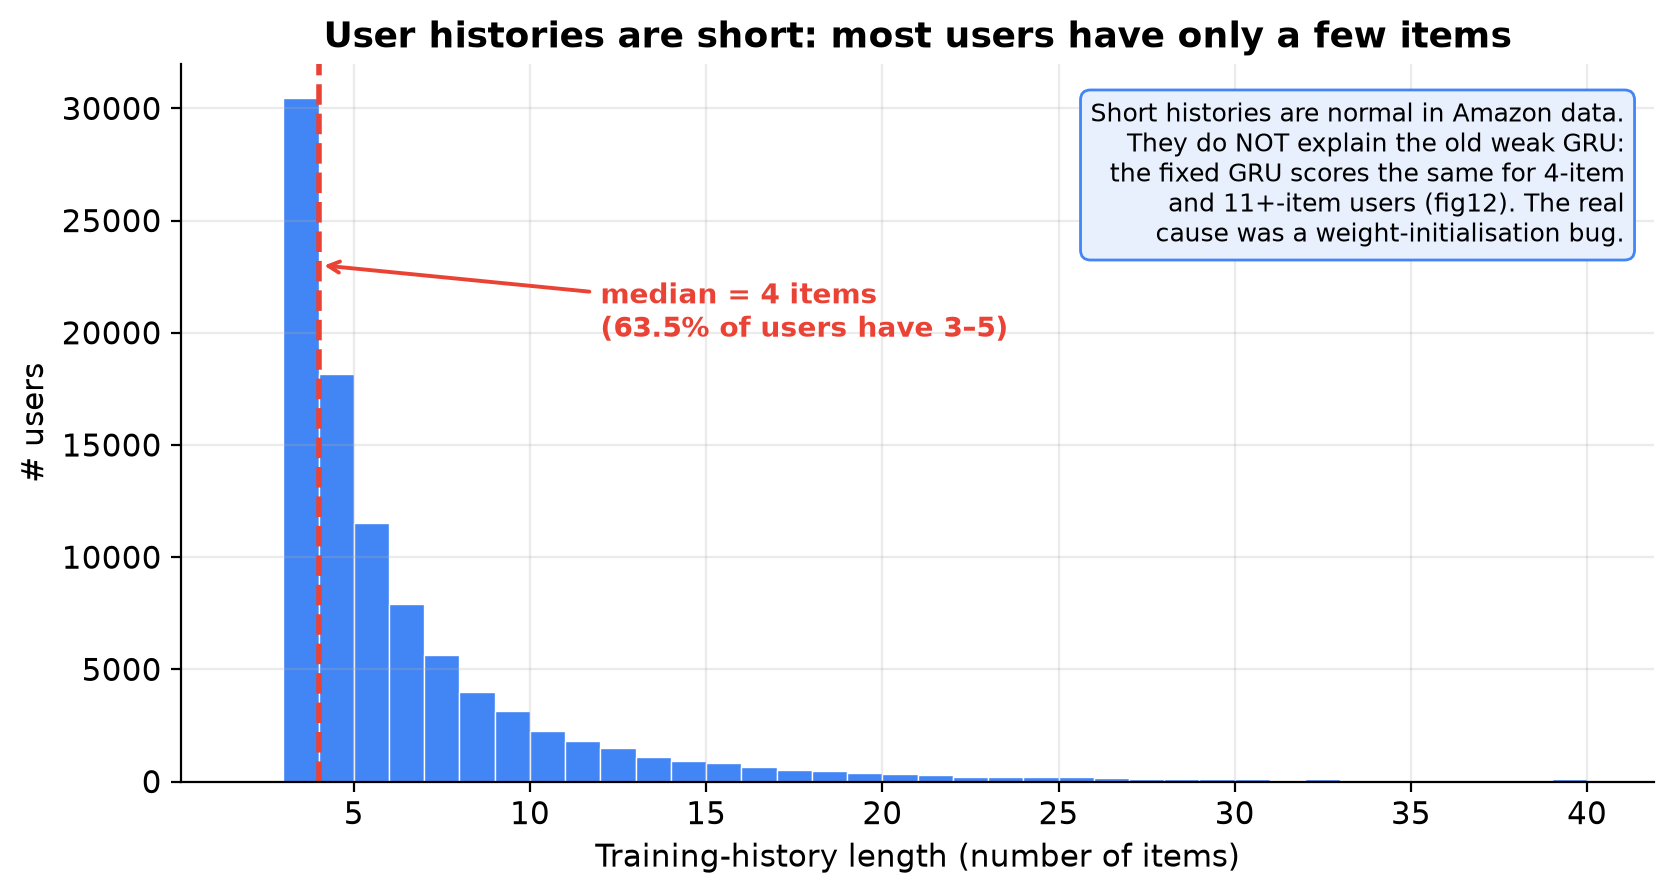
\includegraphics[width=0.78\linewidth]{fig08_history_lengths.png}
  \caption{Distribution of training-history length per user. The median user has four
  training interactions.}
  \label{fig:hist}
\end{figure}

% ================================================================ 4 protocol
\section{Evaluation Protocol}
\label{sec:protocol}

\subsection{Frozen candidate lists}

For each validation and test user we build one 20-item candidate list: the true held-out target
plus 19 negatives sampled without replacement (seed 42) from the 25{,}527 training-vocabulary
items, with probability proportional to training interaction count, excluding everything the
user interacted with in any split. The list is shuffled, hashed and frozen before any system is
evaluated. Every system ranks exactly this list.

This design isolates \emph{ranking} from \emph{retrieval}: if each system retrieved its own
candidates, a retrieval miss would score zero and the comparison would conflate the two stages.
Popularity-proportional sampling makes negatives roughly as popular as targets (on average
$1.01\times$ on validation and $1.40\times$ on test), so global popularity carries no free
signal. A uniformly random permutation has expected Hit@5 of exactly $0.25$, a useful sanity
anchor.

\subsection{Users}

LLM systems are expensive, so all systems are compared on the \emph{same} 100 randomly sampled
test users (and 100 validation users for tuning). Non-LLM systems are additionally evaluated on
all 94{,}762 test users, which gives near-deterministic estimates for them.

\subsection{Metrics}

With a single relevant item per user at rank $r\in\{1,\dots,20\}$,
\begin{equation}
  \Hit@K = \mathbb{1}[r\le K],\qquad
  \NDCG@K = \frac{\mathbb{1}[r\le K]}{\log_2(r+1)},\qquad
  \MRR = \frac{1}{r},
\end{equation}
averaged over users. Hit@5 and NDCG@5 are primary; we also report Hit@10, NDCG@10 and MRR.

\subsection{Statistical testing}

For two systems $A$ and $B$ evaluated on the same users we resample users with replacement
10{,}000 times and report the mean per-user difference with its 95\% percentile interval
\citep{efron1993bootstrap}. A contrast is called significant when the interval excludes zero.
All hyperparameters are tuned on validation users only; the test set is never used for any
selection.

% ================================================================ 5 method
\section{Methods}
\label{sec:method}

\subsection{System overview}

\Cref{fig:arch} shows the overall architecture. A data layer produces sequences and frozen lists;
three families of rankers score each list; a fusion layer optionally blends an LLM ranking with a
trained-model ranking; and an evaluation layer computes metrics and bootstrap intervals from the
saved per-user rankings.

\begin{figure}[htbp]
\centering
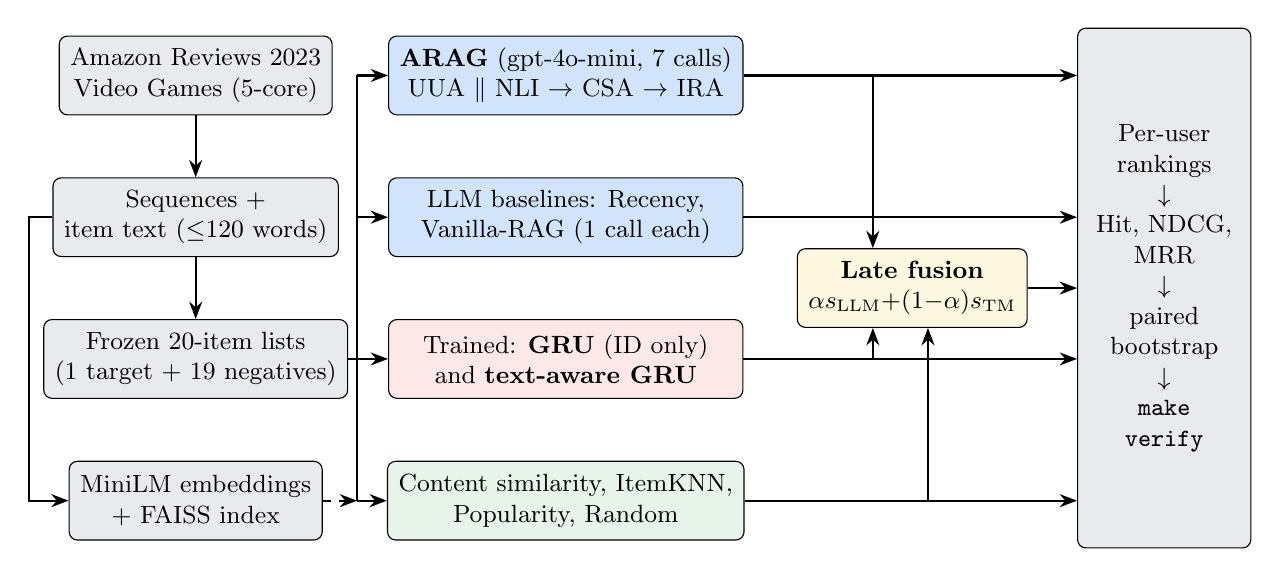
\begin{tikzpicture}
  % data layer (x = 1.5)
  \node[box, fill=cdata, minimum width=3.0cm] (raw)   at (1.5, 0.0)  {Amazon Reviews 2023\\Video Games (5-core)};
  \node[box, fill=cdata, minimum width=3.0cm] (seq)   at (1.5,-1.8)  {Sequences +\\item text ($\le$120 words)};
  \node[box, fill=cdata, minimum width=3.0cm] (lists) at (1.5,-3.6)  {Frozen 20-item lists\\(1 target + 19 negatives)};
  \node[box, fill=cdata, minimum width=3.0cm] (emb)   at (1.5,-5.4)  {MiniLM embeddings\\+ FAISS index};
  \draw[arr] (raw) -- (seq);
  \draw[arr] (seq) -- (lists);
  \draw[arr] (seq.west) -- ++(-0.3,0) |- (emb.west);
  % rankers (x = 6.1)
  \node[box, fill=cllm,  minimum width=4.5cm] (arag) at (6.2, 0.0) {\textbf{ARAG} (gpt-4o-mini, 7 calls)\\UUA $\parallel$ NLI $\to$ CSA $\to$ IRA};
  \node[box, fill=cllm,  minimum width=4.5cm] (llmb) at (6.2,-1.8) {LLM baselines: Recency,\\Vanilla-RAG (1 call each)};
  \node[box, fill=cdl,   minimum width=4.5cm] (gru)  at (6.2,-3.6) {Trained: \textbf{GRU} (ID only)\\and \textbf{text-aware GRU}};
  \node[box, fill=cbase, minimum width=4.5cm] (base) at (6.2,-5.4) {Content similarity, ItemKNN,\\Popularity, Random};
  \coordinate (bus) at (3.55,0);
  \draw[thick] (lists.east) -- (bus |- lists.east);
  \draw[thick] (bus |- arag.west) -- (bus |- base.west);
  \foreach \n in {arag,llmb,gru,base} \draw[arr] (bus |- \n.west) -- (\n.west);
  \draw[arr, dashed] (emb.east) -- (base.west -| bus) ;
  % fusion (x = 10.4) and evaluation (x = 13.6)
  \node[box, fill=cfuse, minimum width=2.6cm] (fuse) at (10.6,-2.7) {\textbf{Late fusion}\\$\alpha s_{\mathrm{LLM}}{+}(1{-}\alpha) s_{\mathrm{TM}}$};
  \node[box, fill=cdata, minimum width=2.2cm, minimum height=6.6cm] (eval) at (13.8,-2.7) {Per-user\\rankings\\$\downarrow$\\Hit, NDCG,\\MRR\\$\downarrow$\\paired\\bootstrap\\$\downarrow$\\\texttt{make}\\\texttt{verify}};
  \foreach \n in {arag,llmb,gru,base} \draw[arr] (\n.east) -- (\n.east -| eval.west);
  \draw[arr] ([xshift=0.35cm]arag.east) -| ([xshift=-0.5cm]fuse.north);
  \draw[arr] ([xshift=0.35cm]gru.east)  -| ([xshift=-0.5cm]fuse.south);
  \draw[arr] ([xshift=0.65cm]base.east) -| ([xshift=0.2cm]fuse.south);
  \draw[arr] (fuse.east) -- (fuse.east -| eval.west);
\end{tikzpicture}
\caption{System architecture. All rankers score the same frozen list. The fusion layer blends
the ARAG ranking with a trained-model or content ranking ($s_{\mathrm{TM}}$); MiniLM embeddings
feed the content baseline and, as item features, the text-aware GRU.}
\label{fig:arch}
\end{figure}

\subsection{ARAG agent pipeline}
\label{sec:arag}

\Cref{fig:arag} details the agentic ranker. Each user's history (training items plus, for test,
the validation item) is rendered as lines of the form \textit{title $\mid$ category $\mid$
rating $\mid$ date}. The long-term context $C_{lt}$ holds up to 50 items and the session context
$C_{st}$ the last five.

\begin{itemize}
  \item \textbf{UUA} (User Understanding Agent, 1 call): from $C_{lt}$ and $C_{st}$, produces
  interests, current intent, dislikes and a summary of at most 120 words, $S_{\mathrm{user}}$.
  \item \textbf{NLI} (4 calls of 5 candidates): for every candidate, a label
  (\textit{support}/\textit{neutral}/\textit{contradict}), a compatibility score in $[0,10]$ and a
  rationale, judged against the raw history.
  \item \textbf{CSA} (Context Summary Agent, 1 call): summarises the accepted candidates
  $\mathcal{I}^+=\{i : \mathrm{score}_i \ge \theta\}$ in at most 200 words, $S_{\mathrm{ctx}}$.
  If no candidate passes $\theta$, the top three by score are used and the fallback is counted.
  \item \textbf{IRA} (Item Ranker Agent, 1 call): given $S_{\mathrm{user}}$, $S_{\mathrm{ctx}}$
  and all 20 candidates, outputs a full permutation $\pi_{\mathrm{LLM}}$ with reasons.
\end{itemize}

UUA and NLI run in parallel. All outputs are requested as strict JSON schemas and validated. A
ranking parser repairs malformed permutations (drops unknown IDs, removes duplicates, appends
missing IDs by NLI score) and counts every repair. Two ablations follow the paper: \emph{ARAG
w/o NLI} (CSA summarises all 20 candidates) and \emph{ARAG w/o NLI \& CSA} (IRA receives only
$S_{\mathrm{user}}$ and the raw candidates).

\begin{figure}[htbp]
\centering
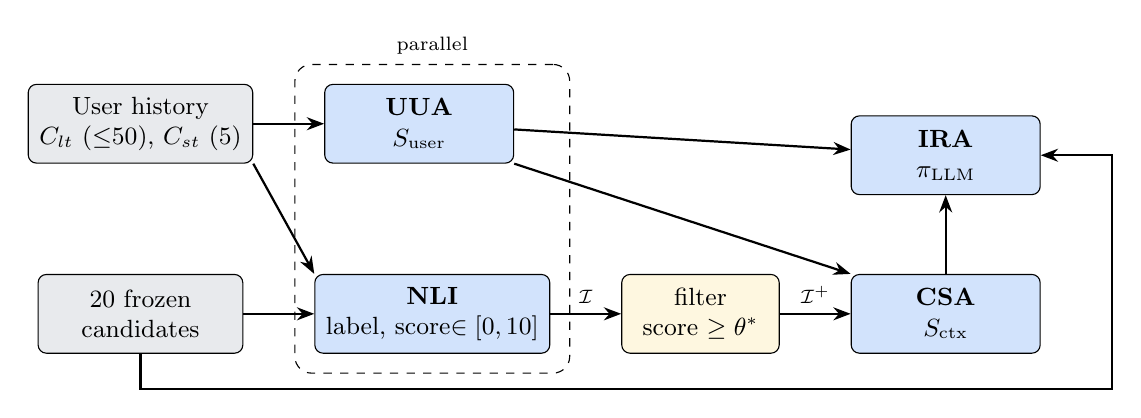
\begin{tikzpicture}[node distance=0.5cm and 0.9cm]
  \node[box, fill=cdata, minimum width=2.6cm] (hist) {User history\\$C_{lt}$ ($\le$50), $C_{st}$ (5)};
  \node[box, fill=cdata, minimum width=2.6cm, below=1.4cm of hist] (cand) {20 frozen\\candidates};
  \node[box, fill=cllm, minimum width=2.4cm, right=of hist] (uua) {\textbf{UUA}\\$S_{\mathrm{user}}$};
  \node[box, fill=cllm, minimum width=2.4cm, right=of cand] (nli) {\textbf{NLI}\\label, score$\in[0,10]$};
  \node[box, fill=cfuse, minimum width=2.0cm, right=of nli] (thr) {filter\\score $\ge\theta^*$};
  \node[box, fill=cllm, minimum width=2.4cm, right=of thr] (csa) {\textbf{CSA}\\$S_{\mathrm{ctx}}$};
  \node[box, fill=cllm, minimum width=2.4cm, above=1.0cm of csa] (ira) {\textbf{IRA}\\$\pi_{\mathrm{LLM}}$};
  \draw[arr] (hist) -- (uua);
  \draw[arr] (hist.south east) -- (nli.north west);
  \draw[arr] (cand) -- (nli);
  \draw[arr] (nli) -- node[above, font=\scriptsize]{$\mathcal{I}$} (thr);
  \draw[arr] (thr) -- node[above, font=\scriptsize]{$\mathcal{I}^+$} (csa);
  \draw[arr] (uua) -- (ira);
  \draw[arr] (uua.south east) -- (csa.north west);
  \draw[arr] (csa) -- (ira);
  \draw[arr] (cand.south) -- ++(0,-0.45) -| ([xshift=0.9cm]csa.east) |- (ira.east);
  \begin{scope}[on background layer]
    \node[grp, fit=(uua)(nli), label={[font=\scriptsize]above:parallel}] {};
  \end{scope}
\end{tikzpicture}
\caption{ARAG agent pipeline (seven LLM calls per user). $\theta^*=5$ is tuned on validation.}
\label{fig:arag}
\end{figure}

\subsection{GRU sequential model}
\label{sec:gru}

Our trained model is a GRU4Rec-style network \citep{hidasi2016session}. Let
$\mathcal{V}$ be the training vocabulary (index 0 = padding, 1 = out-of-vocabulary). For a
history $(i_1,\dots,i_T)$, truncated to the last $T\le 50$ items,
\begin{align}
  \mathbf{x}_t &= \mathrm{Dropout}\big(\mathbf{e}(i_t)\big), &
  \mathbf{h}_t &= \mathrm{GRU}(\mathbf{x}_t, \mathbf{h}_{t-1}), &
  \mathbf{u}_t &= \mathbf{P}\,\mathrm{Dropout}(\mathbf{h}_t),
\end{align}
with $\mathbf{e}(i)\in\mathbb{R}^{64}$, $\mathbf{h}_t\in\mathbb{R}^{d_h}$ and a projection
$\mathbf{P}\in\mathbb{R}^{64\times d_h}$ ($d_h=64$ for the ID-only GRU, 128 for the text-aware GRU). Input and output embeddings are tied: the score of
item $j$ after step $t$ is $\mathbf{u}_t^{\top}\mathbf{e}(j)$. The model is trained with full-softmax
cross-entropy for next-item prediction at every prefix,
\begin{equation}
  \mathcal{L} = -\sum_{u}\sum_{t=1}^{T_u-1}
  \log\frac{\exp\!\big(\mathbf{u}_t^{\top}\mathbf{e}(i_{t+1})\big)}
            {\sum_{j\in\mathcal{V}}\exp\!\big(\mathbf{u}_t^{\top}\mathbf{e}(j)\big)}.
\end{equation}
At inference, the user vector is the final projected state $\mathbf{u}_T$ and candidates are ranked
by $\mathbf{u}_T^{\top}\mathbf{e}(c)$. Item embeddings are initialised from $\mathcal{N}(0,0.02^2)$
with the padding row at zero. This matters with tied embeddings: the default $\mathcal{N}(0,1)$
initialisation makes the initial logits dot products of two unit-variance 64-d vectors
($|\mathbf{u}^{\top}\mathbf{e}|\approx8$), so the softmax over 25{,}527 items is saturated from the
first step and training stalls (\cref{app:initbug}).

\subsection{Text-aware GRU}
\label{sec:textgru}

Most item IDs are seen in few sequences, so their embeddings are estimated from little data. The
text-aware GRU (\cref{fig:textgru}) keeps the network
of \cref{sec:gru} unchanged and replaces only the item representation:
\begin{equation}
  \tilde{\mathbf{e}}(i) = \mathbf{e}(i) + \mathbf{W}\,\mathbf{t}_i,
  \qquad \mathbf{t}_i = \mathrm{MiniLM}(\text{text}_i)\in\mathbb{R}^{384},
  \quad \mathbf{W}\in\mathbb{R}^{64\times384},
  \label{eq:textgru}
\end{equation}
where $\mathbf{t}_i$ is the frozen, L2-normalised \texttt{all-MiniLM-L6-v2} embedding
\citep{reimers2019sentence,wang2020minilm} of the item's metadata, and $\mathbf{W}$ is learned. The
same $\tilde{\mathbf{e}}$ is used for inputs and for the tied output layer, so two items that never
co-occur can still be close because their descriptions are similar. Text features are available
for 25{,}526 of the 25{,}527 vocabulary items; padding and OOV rows are zero.

\begin{figure}[htbp]
\centering
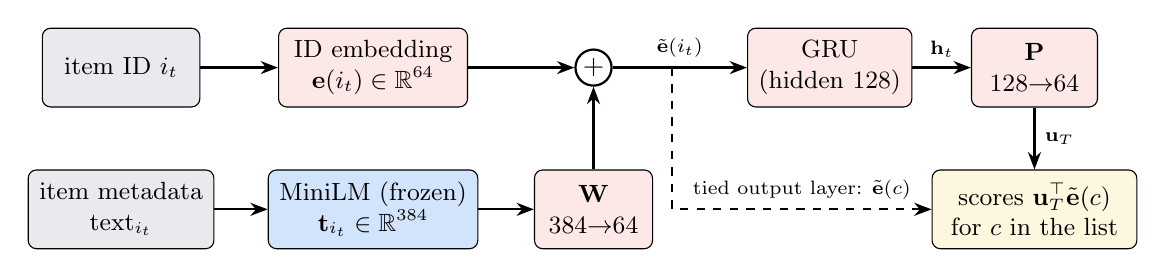
\begin{tikzpicture}
  \node[box, fill=cdata, minimum width=2.0cm] (id)   at (0.0, 0.0) {item ID $i_t$};
  \node[box, fill=cdata, minimum width=2.0cm] (txt)  at (0.0,-1.8) {item metadata\\text$_{i_t}$};
  \node[box, fill=cdl,   minimum width=2.4cm] (eid)  at (3.2, 0.0) {ID embedding\\$\mathbf{e}(i_t)\in\mathbb{R}^{64}$};
  \node[box, fill=cllm,  minimum width=2.4cm] (mini) at (3.2,-1.8) {MiniLM (frozen)\\$\mathbf{t}_{i_t}\in\mathbb{R}^{384}$};
  \node[box, fill=cdl,   minimum width=1.5cm] (W)    at (6.0,-1.8) {$\mathbf{W}$\\384$\to$64};
  \node[draw, circle, thick, inner sep=1pt]   (plus) at (6.0, 0.0) {$+$};
  \node[box, fill=cdl,   minimum width=1.7cm] (gru)  at (9.0, 0.0) {GRU\\(hidden 128)};
  \node[box, fill=cdl,   minimum width=1.6cm] (proj) at (11.6,0.0) {$\mathbf{P}$\\128$\to$64};
  \node[box, fill=cfuse, minimum width=2.6cm] (score) at (11.6,-1.8) {scores $\mathbf{u}_T^{\top}\tilde{\mathbf{e}}(c)$\\for $c$ in the list};
  \draw[arr] (id) -- (eid);
  \draw[arr] (txt) -- (mini);
  \draw[arr] (mini) -- (W);
  \draw[arr] (eid) -- (plus);
  \draw[arr] (W) -- (plus);
  \draw[arr] (plus) -- node[above, font=\scriptsize]{$\tilde{\mathbf{e}}(i_t)$} (gru);
  \draw[arr] (gru) -- node[above, font=\scriptsize]{$\mathbf{h}_t$} (proj);
  \draw[arr] (proj) -- node[right, font=\scriptsize]{$\mathbf{u}_T$} (score);
  \draw[arr, dashed] (7.0,0) |- node[pos=0.75, above, font=\scriptsize]{tied output layer: $\tilde{\mathbf{e}}(c)$} (score.west);
\end{tikzpicture}
\caption{Text-aware GRU. The only change from the ID-only GRU is the item vector
$\tilde{\mathbf{e}}=\mathbf{e}+\mathbf{W}\mathbf{t}$, shared by the input and the tied output layer.}
\label{fig:textgru}
\end{figure}

\subsection{SASRec}
\label{sec:sasrec}

As a second, independent trained baseline we use SASRec \citep{kang2018self}: item embeddings
plus learned position embeddings, two pre-norm Transformer blocks with two heads and a causal
mask, and a final layer norm; the user vector is the output at the last real position. It shares
the GRU's vocabulary, training sequences, tied full-softmax loss, optimiser, early stopping,
initialisation and seeds, so the two trained models differ only in the sequence encoder.

\subsection{Non-learned baselines}

\paragraph{Content similarity.} The user profile is a recency-weighted sum of the history's MiniLM
vectors, $\mathbf{p}_u=\sum_{k=1}^{T} w_k\,\mathbf{t}_{i_k}$ with $w_k=\exp(-d\,(T-k))$, and
candidates are ranked by $\mathbf{p}_u^{\top}\mathbf{t}_c$.

\paragraph{ItemKNN.} From the binary user--item training matrix $\mathbf{X}$ we compute cosine
item--item similarity $\mathrm{sim}(a,b)=\frac{(\mathbf{X}^{\top}\mathbf{X})_{ab}}{\sqrt{n_a n_b}}$
\citep{sarwar2001item}, with $n_a$ the number of users of item $a$, and score candidate $c$ as
$\sum_k w_k\,\mathrm{sim}(i_k,c)$.

\paragraph{Popularity and random.} Candidates ordered by training interaction count, or by a
seeded random permutation.

\paragraph{LLM baselines.} Following the paper, \emph{LLM-Recency} prompts the ranker with the
last ten history items, and \emph{LLM-Vanilla-RAG} with the ten history items most similar to the
mean candidate embedding; each uses one LLM call.

\subsection{Late fusion}
\label{sec:fusion}

An LLM ranker outputs a permutation, not scores, so we fuse rankings. With rank $r_s(i)$ of item
$i$ under system $s$ on a list of $n=20$,
\begin{equation}
  s_s(i) = 1 - \frac{r_s(i)-1}{n-1}, \qquad
  f(i) = \alpha\, s_{\mathrm{LLM}}(i) + (1-\alpha)\, s_{\mathrm{TM}}(i),
  \label{eq:fusion}
\end{equation}
with ties broken by NLI score, then item ID. $\alpha=1$ reproduces ARAG exactly and $\alpha=0$
reproduces the trained model exactly, so the trained model's contribution is exactly ablatable.
$\alpha\in\{0,0.1,\dots,1\}$ is chosen on the 100 validation users. We fuse ARAG with the ID-only
GRU (\emph{ARAG + GRU}, the original proposal), with the text-aware GRU and with content
similarity.

% ================================================================ 6 setup
\section{Experimental Setup}
\label{sec:setup}

\paragraph{Implementation.} Python 3.11 and PyTorch; \texttt{sentence-transformers}
\texttt{all-MiniLM-L6-v2} (384-d, normalised) with a FAISS \citep{johnson2019billion}
inner-product index; FastAPI and React for an interactive demonstrator. The LLM is OpenAI
\texttt{gpt-4o-mini} at temperature 0 with strict JSON-schema outputs. A local
\texttt{qwen3:8b} model via Ollama is supported by the same client and used for the test suite.

\paragraph{Hyperparameters.} \Cref{tab:hparams} lists all settings. The ID-only GRU was selected
from a grid hidden $\in\{64,128\}\times$ dropout $\in\{0.2,0.5\}$ (best: 64/0.2, validation
NDCG@5 $0.531$); SASRec from dropout $\in\{0.2,0.5\}$ (best 0.5, $0.530$). The text-aware GRU
uses hidden 128 and dropout 0.2 without a grid. All trained models use the same 30-epoch cap and
select the checkpoint with the best validation NDCG@5 over all 94{,}762 validation users.

\begin{table}[h]
\centering
\caption{Hyperparameters. All selections use validation data only.}
\label{tab:hparams}
\small
\begin{tabular}{llc}
\toprule
Component & Setting & Value \\
\midrule
Trained models & item dimension; init & 64; $\mathcal{N}(0,0.02^2)$ \\
          & optimiser; learning rate & Adam; $10^{-3}$ \\
          & batch size; max sequence length & 256; 50 \\
          & epochs (max); early-stopping patience & 30; 3 \\
          & seeds & 0, 1, 2 \\
GRU / text-aware GRU & hidden dimension; dropout & 64 / 128; 0.2 \\
SASRec & blocks; heads; dropout & 2; 2; 0.5 \\
Text-aware GRU & text encoder (frozen); projection & MiniLM-L6-v2; 384$\to$64 \\
ARAG & NLI acceptance threshold $\theta^*$ (grid 4--7) & 5 \\
     & candidates per NLI call; temperature & 5; 0 \\
Fusion & $\alpha^*$: ARAG+GRU / +text-GRU / +content & 0.2 / 0.1 / 0.4 \\
Content, ItemKNN & recency decay $d^*$ (grid 0, 0.3, 0.6, 1.0) & 0.3 / 0.3 \\
Lists & size; negatives; sampling seed & 20; 19; 42 \\
Bootstrap & resamples; interval & 10{,}000; 95\% percentile \\
\bottomrule
\end{tabular}
\end{table}

\paragraph{Tuning.} Validation NDCG@5 for the NLI threshold was $\theta=4$: 0.4228, $\theta=5$: 0.4305, $\theta=6$: 0.3993, $\theta=7$: 0.3962
, giving
$\theta^*=5$. \Cref{tab:alpha} shows the validation $\alpha$ curves.

\paragraph{Cost and reproducibility.} Every LLM response is stored in a disk cache keyed by the
hash of (model, prompt, schema). The corrected evaluation made 2{,}263 new calls (about
\$1.06); total unique project spend across both protocol versions was 4{,}668 calls, 10.3\,M input
and 0.83\,M output tokens, \$2.04. With \texttt{REPLAY\_ONLY=1}, any uncached call raises an
error, so all later experiments (content baselines, text-aware GRU, the corrected GRU, SASRec
and new fusions) were evaluated at a guaranteed cost of \$0. A verification script recomputes every metric from the
saved per-user rankings and checks dataset and list hashes against the run record.

\paragraph{Compute.} All training ran on a laptop CPU (Apple silicon, 16\,GB RAM). The ID-only GRU
grid and seeds took about 2\,h\,25\,min, the text-aware GRU about 9\,min per seed and SASRec about
15\,min per seed, after two memory optimisations (logits computed only at non-padded positions;
chunked validation) that do not change the loss.

% ================================================================ 7 results
\section{Results}
\label{sec:results}

\subsection{Main comparison}

\Cref{tab:main} reports every system on the same 100 test users, and \cref{tab:allusers} the
non-LLM systems on all 94{,}762 test users. \Cref{tab:paired} gives the paired contrasts.

\begin{table}[htbp]
\centering
\caption{All systems on the same 100 sampled test users (best value per column in bold).
Trained models are shown per seed. Standard deviations across users are about 0.4--0.5 for Hit
and 0.3--0.45 for NDCG; see \cref{tab:paired} for paired confidence intervals.}
\label{tab:main}
\small
\begin{tabular}{lccccc}
\toprule
System & Hit@5 & NDCG@5 & Hit@10 & NDCG@10 & MRR \\
\midrule
\multicolumn{6}{l}{\textit{Non-learned}} \\
\quad Random & 0.220 & 0.125 & 0.470 & 0.205 & 0.162 \\
\quad Popularity & 0.200 & 0.109 & 0.470 & 0.197 & 0.150 \\
\quad Content similarity & 0.590 & 0.439 & 0.820 & 0.510 & 0.429 \\
\quad ItemKNN & 0.540 & 0.399 & 0.670 & 0.442 & 0.392 \\
\midrule
\multicolumn{6}{l}{\textit{Trained sequential models}} \\
\quad GRU, ID only (seed 0) & 0.680 & 0.519 & 0.850 & 0.575 & 0.499 \\
\quad GRU, ID only (seed 1) & \textbf{0.720} & 0.526 & 0.840 & 0.563 & 0.487 \\
\quad GRU, ID only (seed 2) & 0.690 & 0.515 & 0.850 & 0.565 & 0.486 \\
\quad Text-aware GRU (seed 0) & \textbf{0.720} & 0.506 & 0.900 & 0.565 & 0.465 \\
\quad Text-aware GRU (seed 1) & 0.700 & 0.497 & 0.900 & 0.562 & 0.463 \\
\quad Text-aware GRU (seed 2) & 0.700 & 0.499 & \textbf{0.910} & 0.568 & 0.468 \\
\midrule
\multicolumn{6}{l}{\textit{LLM baselines and ablations}} \\
\quad LLM-Recency & 0.400 & 0.285 & 0.630 & 0.358 & 0.300 \\
\quad LLM-Vanilla-RAG & 0.380 & 0.263 & 0.670 & 0.355 & 0.283 \\
\quad ARAG w/o NLI \& CSA & 0.470 & 0.362 & 0.630 & 0.414 & 0.372 \\
\quad ARAG w/o NLI & 0.510 & 0.376 & 0.720 & 0.445 & 0.380 \\
\midrule
\multicolumn{6}{l}{\textit{Agentic LLM and fusion}} \\
\quad ARAG & 0.530 & 0.424 & 0.700 & 0.479 & 0.432 \\
\quad ARAG + GRU & 0.690 & 0.523 & 0.840 & 0.574 & \textbf{0.502} \\
\quad ARAG + content & 0.590 & 0.423 & 0.810 & 0.494 & 0.411 \\
\quad ARAG + text-aware GRU & \textbf{0.720} & \textbf{0.532} & \textbf{0.910} & \textbf{0.594} & 0.501 \\
\bottomrule
\end{tabular}

\end{table}

\begin{table}[htbp]
\centering
\caption{Non-LLM systems on all 94{,}762 test users (mean $\pm$ standard deviation over three
seeds for the GRUs).}
\label{tab:allusers}
\begin{tabular}{lccc}
\toprule
System & Hit@5 & NDCG@5 & MRR \\
\midrule
Random & 0.252 & 0.149 & 0.181 \\
Popularity & 0.213 & 0.128 & 0.166 \\
ItemKNN & 0.519 & 0.406 & 0.406 \\
Content similarity & 0.569 & 0.411 & 0.402 \\
GRU, ID only (3 seeds) & 0.686 $\pm$ 0.001 & 0.505 $\pm$ 0.001 & 0.478 $\pm$ 0.000 \\
Text-aware GRU (3 seeds) & \textbf{0.716 $\pm$ 0.001} & \textbf{0.530 $\pm$ 0.001} & \textbf{0.500 $\pm$ 0.002} \\
\bottomrule
\end{tabular}

\end{table}

\begin{table}[htbp]
\centering
\caption{Paired bootstrap contrasts on the same 100 test users ($\Delta$NDCG@5, 95\% CI,
10{,}000 resamples). GRU and text-aware GRU refer to seed 0 unless stated. H1$'$/H2$'$ repeat
H1/H2 with the text-aware GRU.}
\label{tab:paired}
\small
\begin{tabular}{lrcc}
\toprule
Contrast & $\Delta$NDCG@5 & 95\% CI & Sig. \\
\midrule
\textbf{H1}: ARAG + GRU $-$ ARAG & $+0.098$ & $[+0.013, +0.182]$ & yes \\
\textbf{H2}: ARAG + GRU $-$ GRU & $+0.004$ & $[-0.038, +0.045]$ & no \\
ARAG $-$ LLM-Recency & $+0.139$ & $[+0.063, +0.217]$ & yes \\
ARAG $-$ LLM-Vanilla-RAG & $+0.162$ & $[+0.079, +0.247]$ & yes \\
ARAG $-$ ARAG w/o NLI & $+0.049$ & $[-0.011, +0.111]$ & no \\
ARAG $-$ ARAG w/o NLI \& CSA & $+0.062$ & $[+0.016, +0.113]$ & yes \\
ARAG $-$ GRU (seed 1) & $-0.101$ & $[-0.201, +0.001]$ & no \\
ARAG $-$ Popularity & $+0.315$ & $[+0.224, +0.408]$ & yes \\
\midrule
Text-aware GRU $-$ GRU & $-0.013$ & $[-0.064, +0.039]$ & no \\
Text-aware GRU $-$ ARAG & $+0.081$ & $[-0.016, +0.179]$ & no \\
Content similarity $-$ ARAG & $+0.014$ & $[-0.088, +0.116]$ & no \\
ItemKNN $-$ ARAG & $-0.025$ & $[-0.132, +0.082]$ & no \\
\textbf{H1$'$}: ARAG + text-GRU $-$ ARAG & $+0.108$ & $[+0.016, +0.197]$ & yes \\
\textbf{H2$'$}: ARAG + text-GRU $-$ text-GRU & $+0.026$ & $[-0.001, +0.054]$ & no \\
ARAG + content $-$ ARAG & $-0.001$ & $[-0.070, +0.066]$ & no \\
\bottomrule
\end{tabular}

\end{table}

\paragraph{Overview.} ARAG is the best LLM-based system (NDCG@5 $0.424$): it significantly beats
LLM-Recency ($+0.139$), LLM-Vanilla-RAG ($+0.162$) and popularity ($+0.315$). The trained
sequential models are more accurate still: on the same users the GRU reaches $0.519$ (seed 0),
SASRec $0.536$ and the fused ARAG + text-GRU $0.532$. \Cref{fig:main} visualises the comparison
and \cref{fig:hyp} the hypothesis tests.

\begin{figure}[htbp]
  \centering
  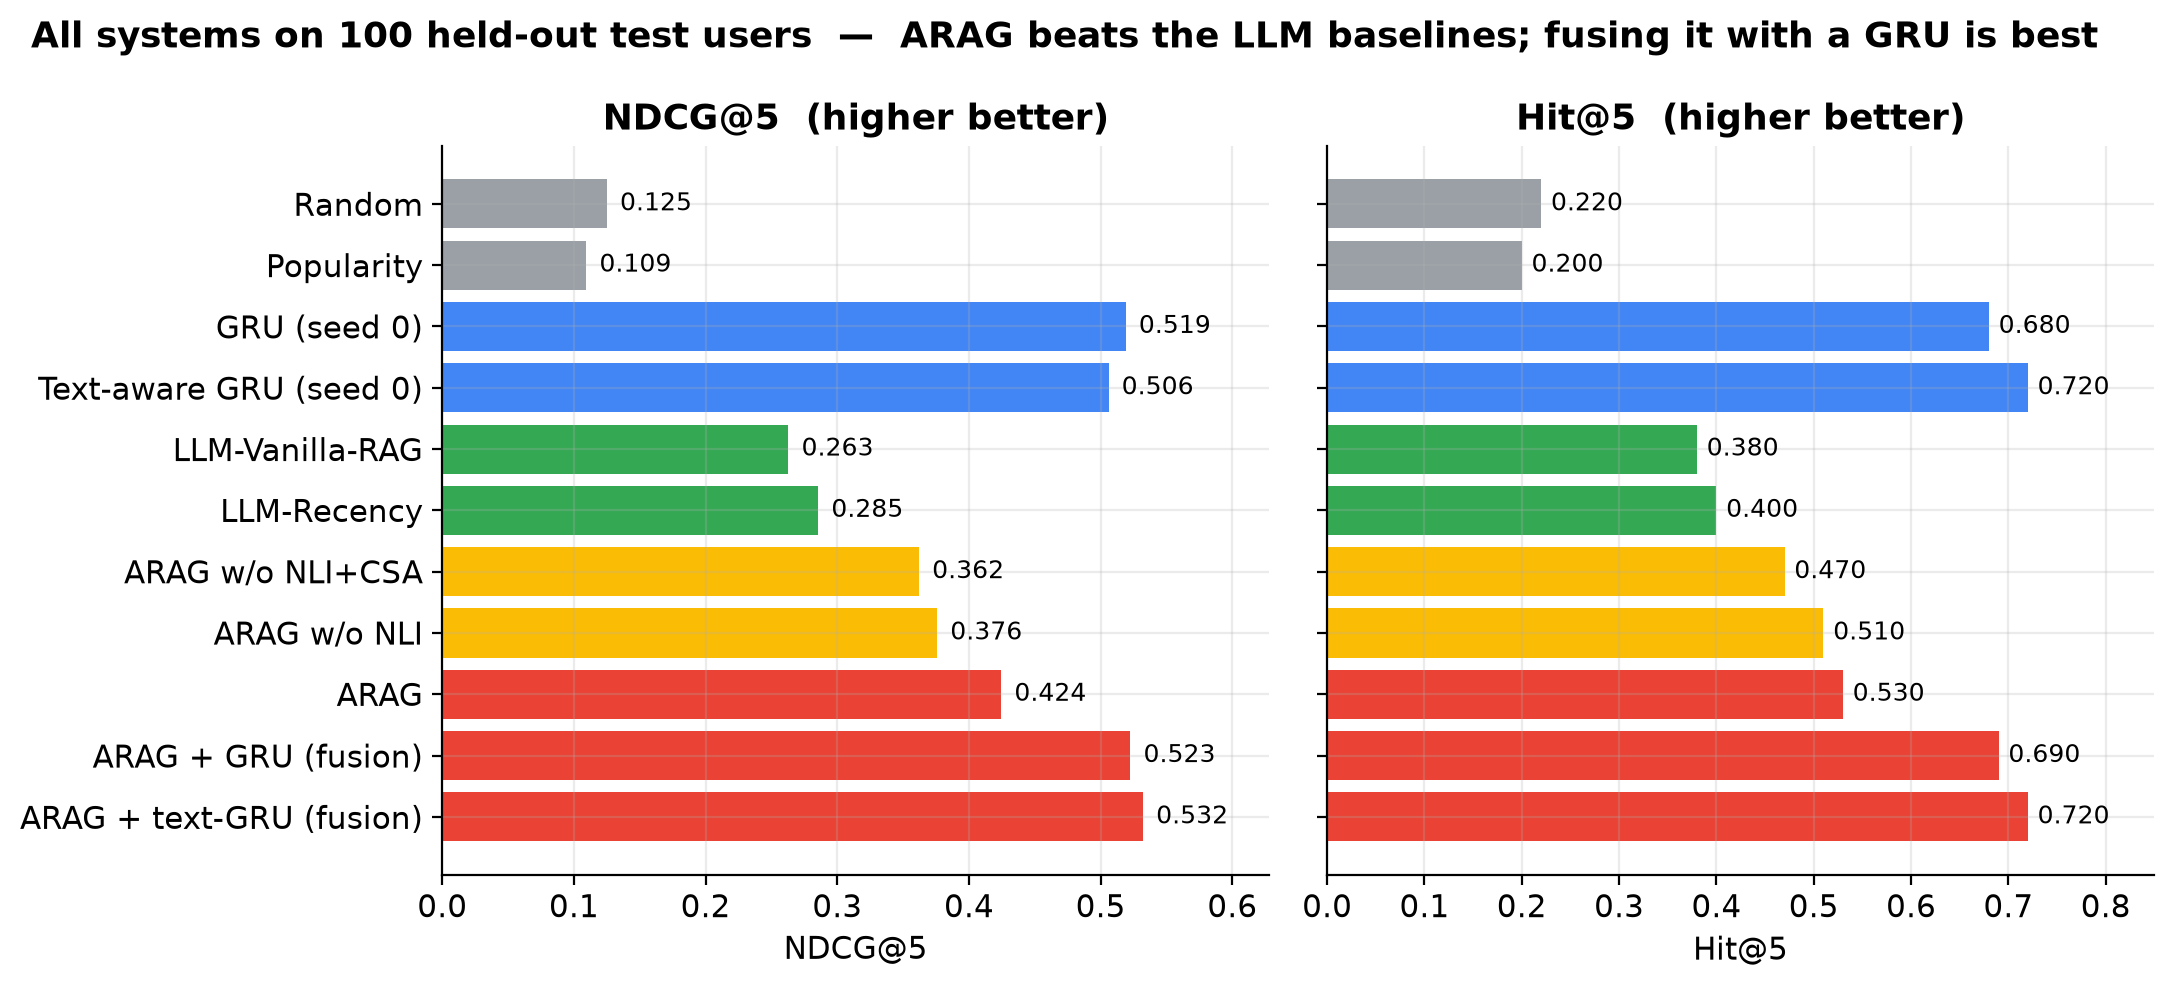
\includegraphics[width=0.9\linewidth]{fig02_main_results.png}
  \caption{NDCG@5 and Hit@5 on the 100 test users.}
  \label{fig:main}
\end{figure}

\begin{figure}[htbp]
  \centering
  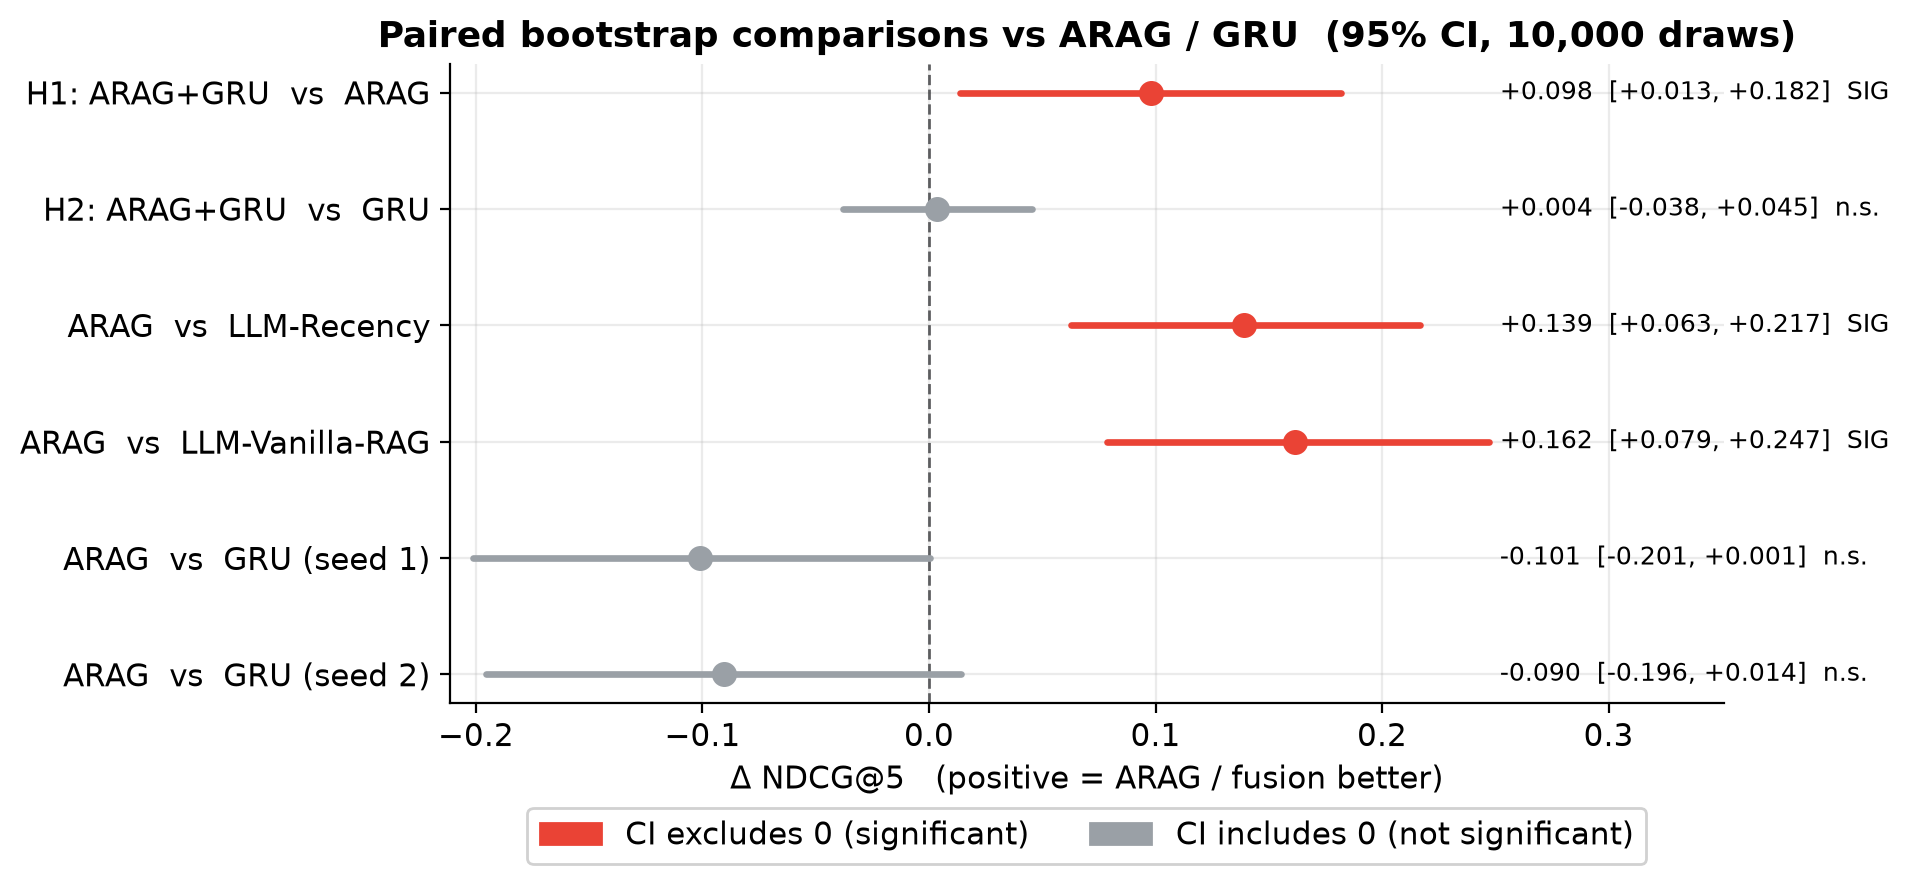
\includegraphics[width=0.85\linewidth]{fig03_hypotheses.png}
  \caption{Forest plot of the key contrasts ($\Delta$NDCG@5, 95\% CI).}
  \label{fig:hyp}
\end{figure}

\subsection{RQ1: does fusing the GRU help ARAG?}

\textbf{H1 is supported.} At the validation-optimal $\alpha^*=0.2$, ARAG + GRU improves NDCG@5 over
ARAG by $+0.098$ $[+0.013,+0.182]$. \textbf{H2 is not supported}: the fused system is no better
than the GRU alone ($+0.004$ $[-0.038,+0.045]$). \Cref{fig:alpha} and \cref{tab:alpha} show the
shape: validation and test both peak at small $\alpha$ (mostly GRU) and fall steadily towards
pure ARAG. Adding a little of ARAG's ranking is harmless or slightly helpful; giving it most of the
weight costs about $0.1$ NDCG@5. With the text-aware GRU the picture is the same (H1$'$:
$+0.108$, significant; H2$'$: $+0.026$, n.s.\ for seed 0, $+0.031$ $[+0.002,+0.061]$ against the
three-seed average).

\begin{figure}[htbp]
  \centering
  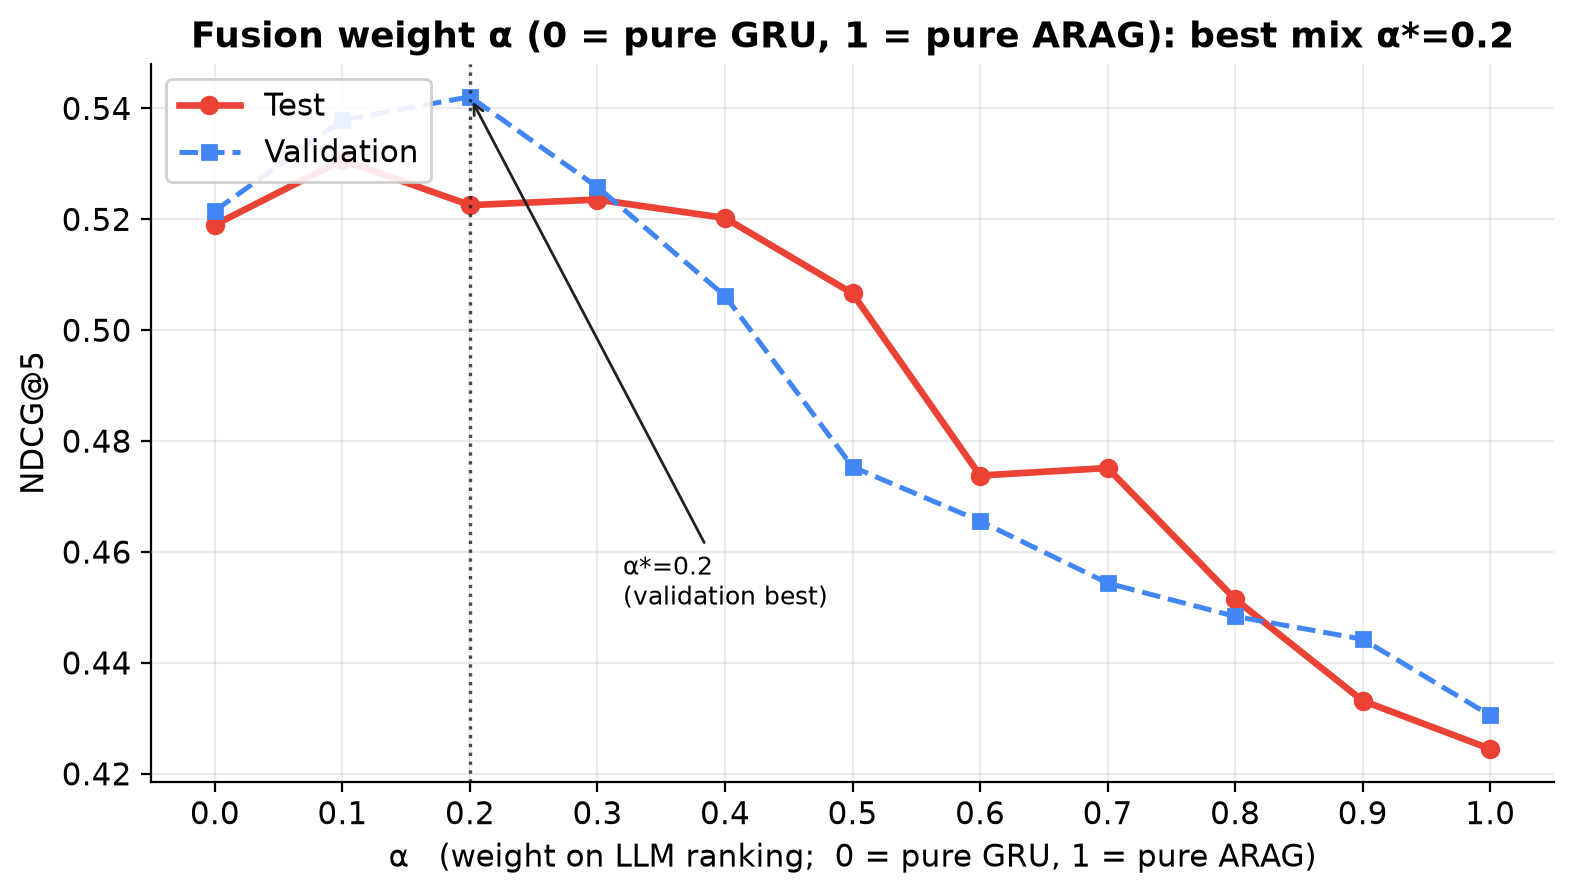
\includegraphics[width=0.75\linewidth]{fig05_alpha_curve.png}
  \caption{NDCG@5 of ARAG + GRU as a function of the fusion weight $\alpha$ (0 = GRU only,
  1 = ARAG only).}
  \label{fig:alpha}
\end{figure}

\begin{table}[htbp]
\centering
\caption{NDCG@5 against the fusion weight $\alpha$ ($\alpha^*$ in bold where it falls on a
shown grid point; for ARAG + GRU, $\alpha^*=0.2$; for ARAG + text-GRU, $\alpha^*=0.1$). Validation curves are on the 100
validation users.}
\label{tab:alpha}
\small
\begin{tabular}{lcccccccc}
\toprule
$\alpha$ & 0.0 & 0.2 & 0.3 & 0.4 & 0.6 & 0.8 & 0.9 & 1.0 \\
\midrule
ARAG + GRU, validation & 0.522 & \textbf{0.542} & 0.526 & 0.506 & 0.466 & 0.448 & 0.444 & 0.431 \\
ARAG + GRU, test & 0.519 & 0.523 & 0.524 & 0.520 & 0.474 & 0.451 & 0.433 & 0.424 \\
ARAG + text-GRU, validation & 0.557 & 0.551 & 0.538 & 0.522 & 0.463 & 0.453 & 0.440 & 0.431 \\
ARAG + content, validation & 0.441 & 0.451 & 0.465 & \textbf{0.489} & 0.455 & 0.451 & 0.438 & 0.431 \\
\bottomrule
\end{tabular}

\end{table}

As an exploratory, post-hoc analysis on the test users (not used for any selection),
\cref{fig:fusionrules} compares the linear rank transform of \cref{eq:fusion} with reciprocal-rank
fusion and an exponential transform. The best points ($0.531$--$0.546$) differ by less than the
confidence intervals of \cref{tab:paired}.

\begin{figure}[htbp]
  \centering
  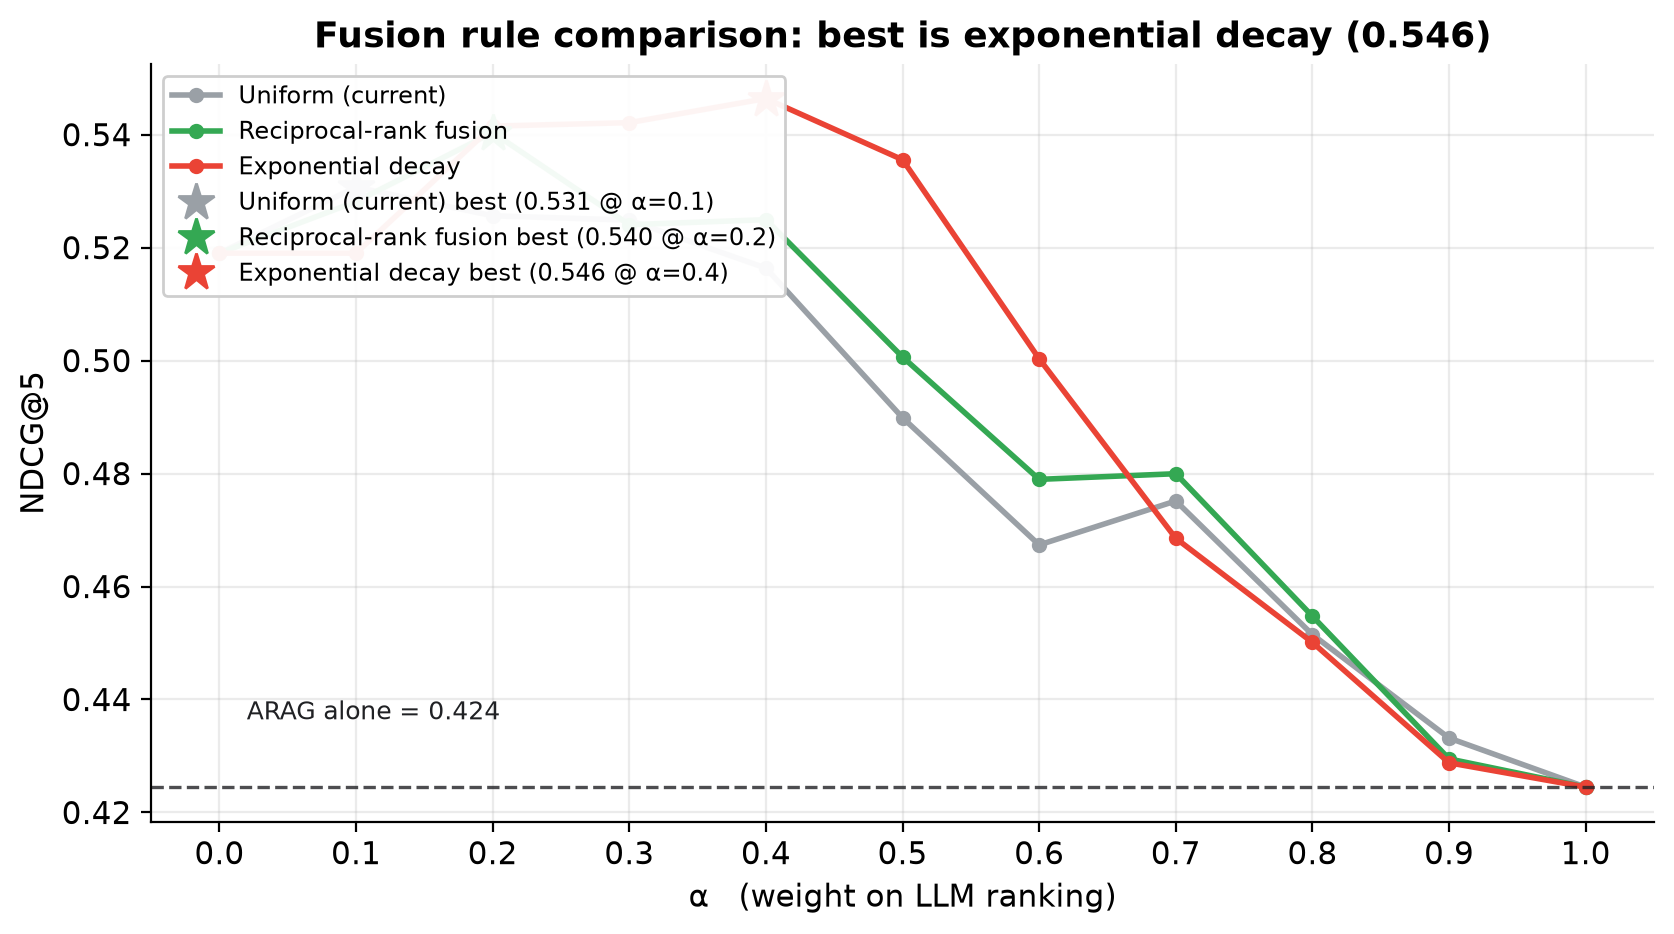
\includegraphics[width=0.75\linewidth]{fig09_fusion_methods.png}
  \caption{Exploratory comparison of rank-to-score transforms for ARAG + ID-only GRU on the
  test users. Shown for completeness; selecting a rule on these numbers would leak test data.}
  \label{fig:fusionrules}
\end{figure}

\subsection{RQ2: do the paper's claims hold?}

Both of the paper's baseline orderings reproduce significantly
(\cref{tab:paired}), and the ablation staircase has the same shape as in all three of the paper's
categories (\cref{fig:abl}): removing NLI and CSA significantly hurts ($-0.062$
$[-0.113,-0.016]$), and removing NLI alone is directionally negative but not significant
($-0.049$ $[-0.111,+0.011]$). \Cref{fig:paper} sets our numbers next to the paper's Table~1.
The absolute values are not comparable (different dataset version, category, model and candidate
protocol), but ARAG's relative lift over the best baseline ($+48.8\%$ NDCG@5) is at least as large
as the paper's ($+25.6\%$ to $+42.1\%$).

\begin{figure}[htbp]
  \centering
  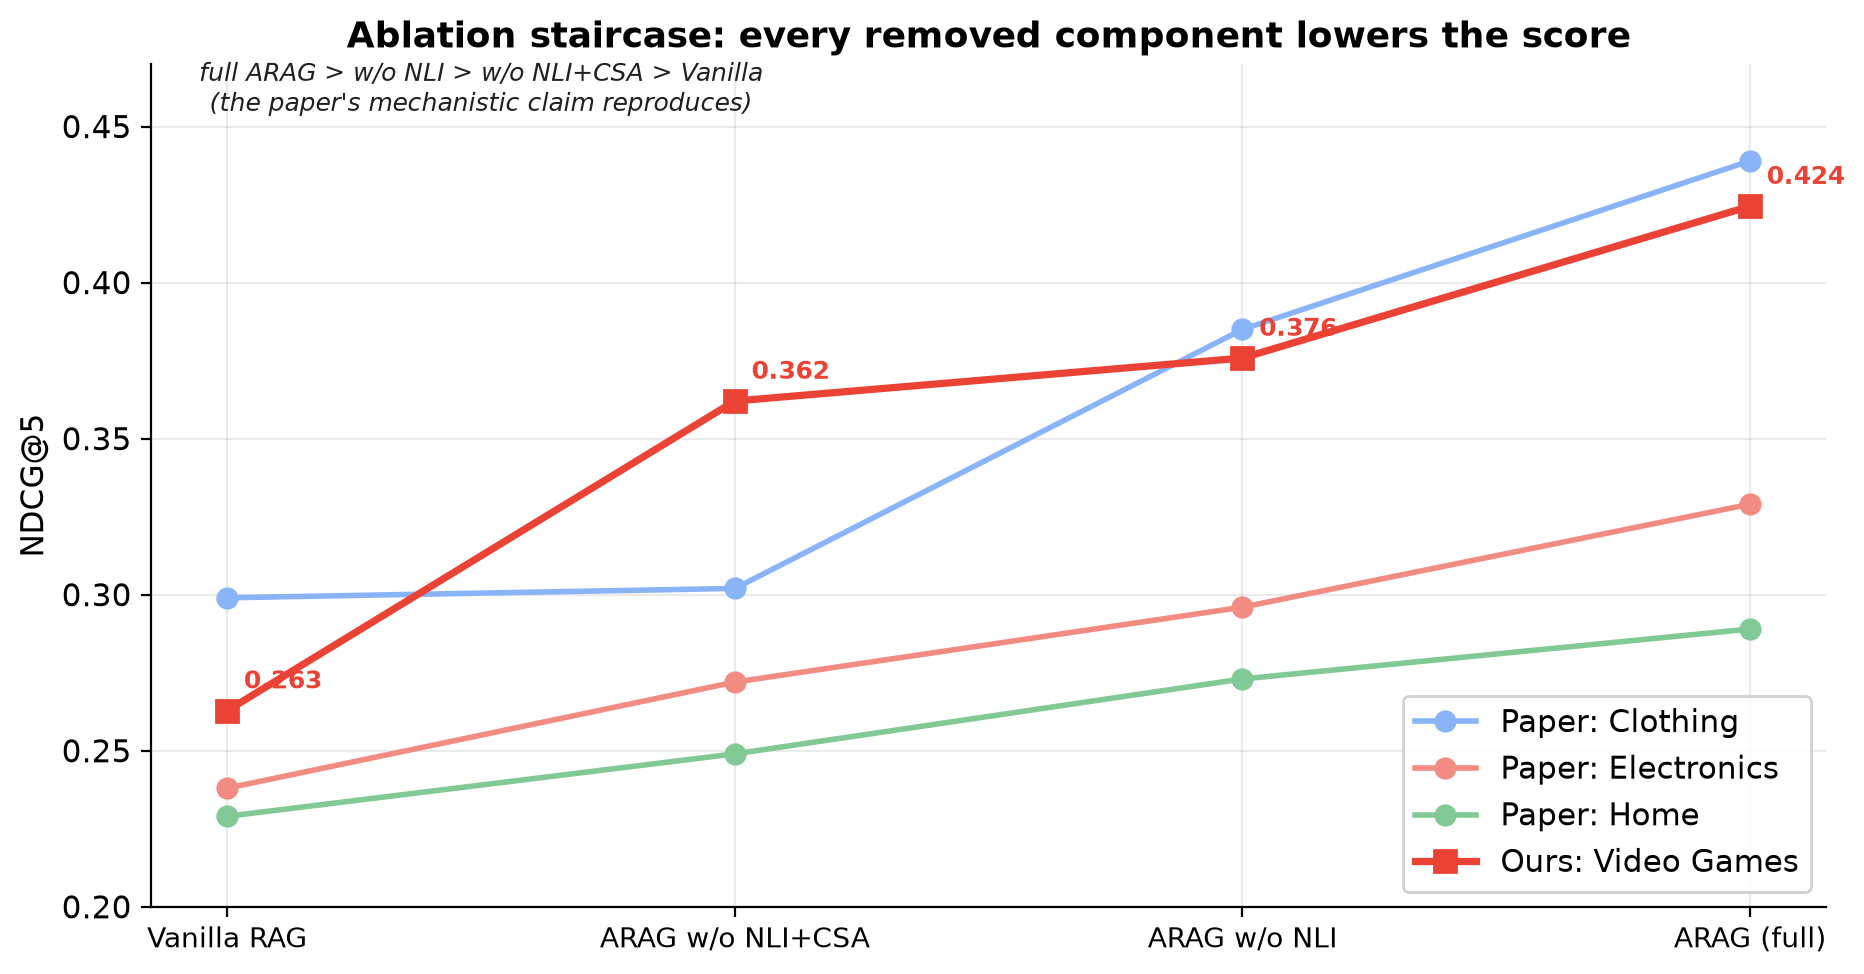
\includegraphics[width=0.8\linewidth]{fig04_ablation.png}
  \caption{Ablation staircase: ours (Video Games) next to the paper's three categories.}
  \label{fig:abl}
\end{figure}

\begin{figure}[htbp]
  \centering
  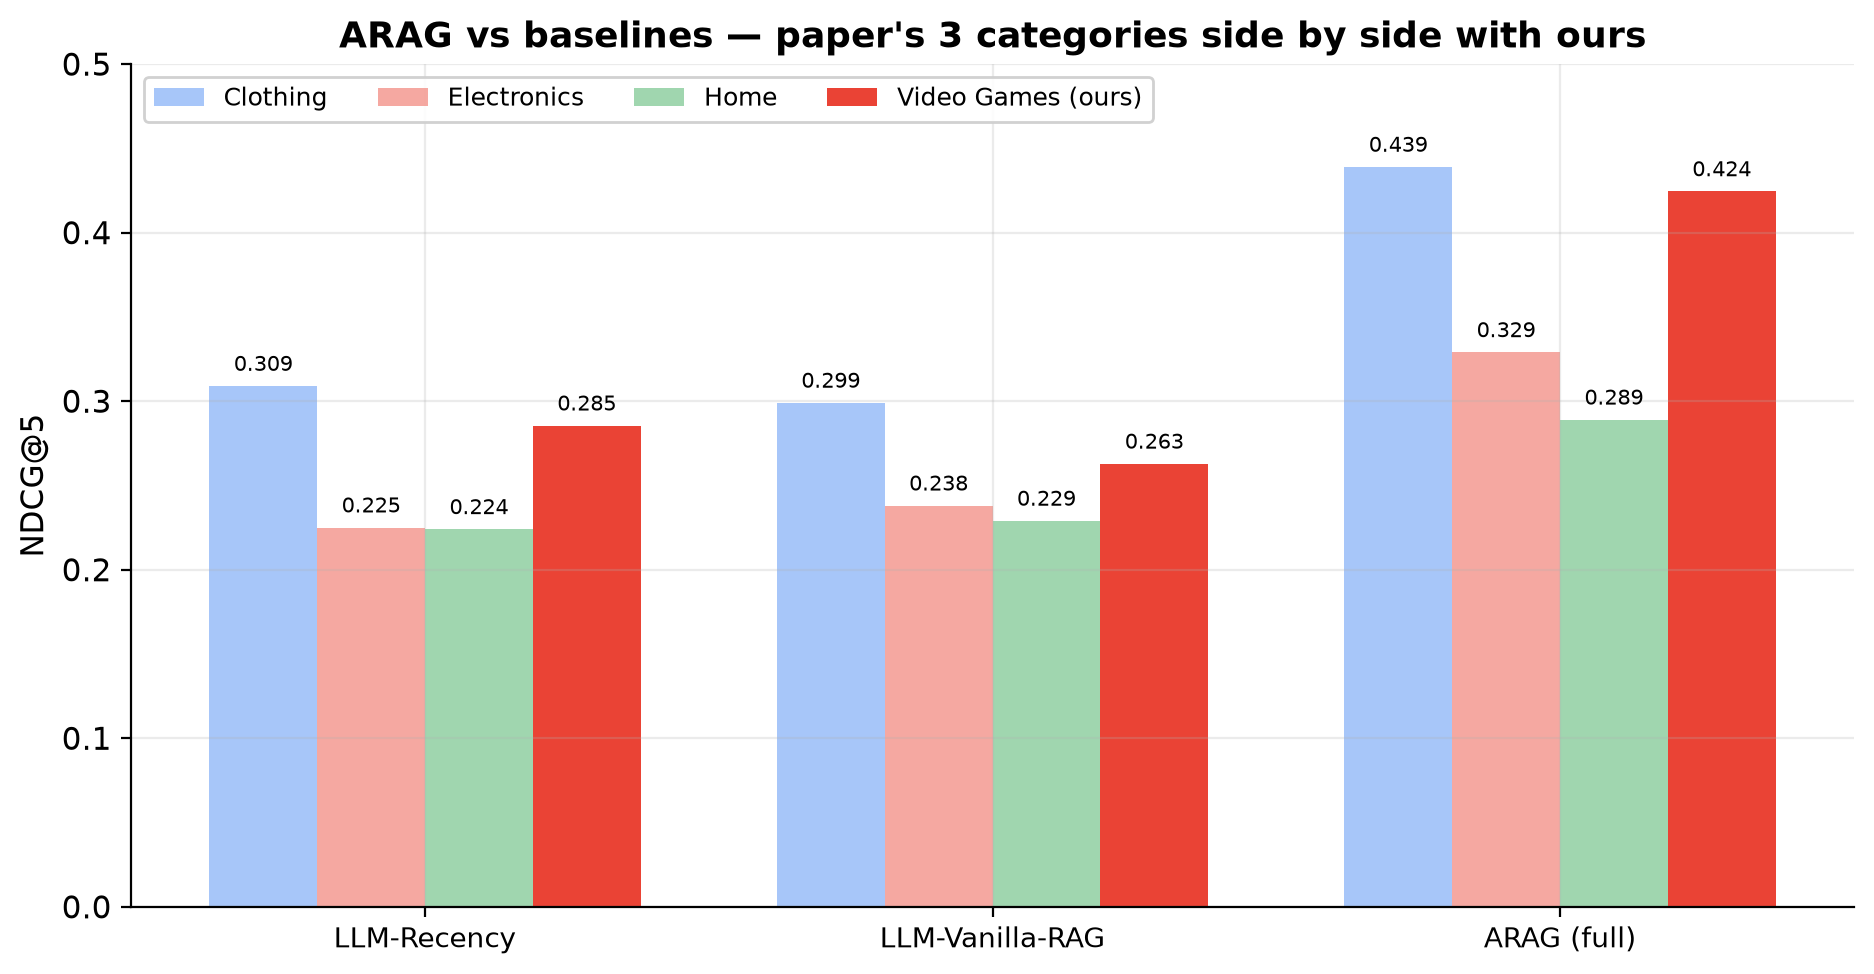
\includegraphics[width=0.85\linewidth]{fig06_paper_vs_ours.png}
  \caption{Our results next to the base paper's Table~1. Absolute values are shown for context
  only; the setups differ in dataset version, category, LLM and candidate construction.}
  \label{fig:paper}
\end{figure}

\subsection{RQ3: trained sequential models}

\Cref{tab:allusers} and \cref{tab:sasrec} report the trained models on all 94{,}762 test users.
The ID-only GRU reaches NDCG@5 $0.505\pm0.001$ and SASRec $0.508$ (three seeds: $0.506$, $0.510$,
$0.506$), a negligible $+0.003$ difference; two different sequence encoders under one protocol land
at the same accuracy. The text-aware GRU is best at $0.530\pm0.001$, $+0.026$ $[+0.024,+0.027]$ over
the ID-only GRU and $+0.120$ $[+0.117,+0.122]$ over content similarity. \Cref{fig:textcurve} shows
that text mainly speeds up learning: the text-aware GRU passes $0.53$ validation NDCG@5 by epoch 4,
the ID-only GRU by epoch 28.

On the 100 LLM users the trained models are all above ARAG (\cref{fig:sasrec}): ARAG $-$ SASRec
$=-0.112$ $[-0.213,-0.009]$ (significant), ARAG $-$ GRU $=-0.095$ $[-0.196,+0.006]$ and ARAG $-$
text-aware GRU $=-0.076$ $[-0.173,+0.021]$ (three-seed averages, not significant at $n=100$).
Test-time sanity checks on SASRec confirm that it uses the user's own history: replacing it with
another user's history drops NDCG@5 from $0.509$ to $0.181$, an empty history gives $0.130$
(near random), and a shuffled history $0.434$. Only 0.4\% of targets and no negatives are out of
vocabulary.

\begin{table}[htbp]
\centering
\caption{Key paired contrasts involving SASRec and ARAG ($\Delta$NDCG@5 $=$ first $-$ second,
95\% CI; $^{*}$ = CI excludes 0). Seeded models are averaged over three seeds per user.}
\label{tab:sasrec}
\small
\begin{tabular}{lrc}
\toprule
Contrast ($\Delta$NDCG@5) & Users & 95\% CI \\
\midrule
SASRec vs GRU (ID) & 94{,}762 & $+0.003$ [$+0.002$, $+0.004$]$^{*}$ \\
SASRec vs Text-aware GRU & 94{,}762 & $-0.023$ [$-0.024$, $-0.021$]$^{*}$ \\
SASRec vs ItemKNN & 94{,}762 & $+0.102$ [$+0.100$, $+0.105$]$^{*}$ \\
ARAG vs SASRec & 100 & $-0.112$ [$-0.213$, $-0.009$]$^{*}$ \\
ARAG vs GRU (ID) & 100 & $-0.095$ [$-0.196$, $+0.006$] \\
ARAG vs Text-aware GRU & 100 & $-0.076$ [$-0.173$, $+0.021$] \\
ARAG + text-GRU vs ARAG & 100 & $+0.108$ [$+0.016$, $+0.197$]$^{*}$ \\
ARAG + text-GRU vs SASRec & 100 & $-0.004$ [$-0.052$, $+0.043$] \\
\bottomrule
\end{tabular}

\end{table}

\begin{figure}[htbp]
  \centering
  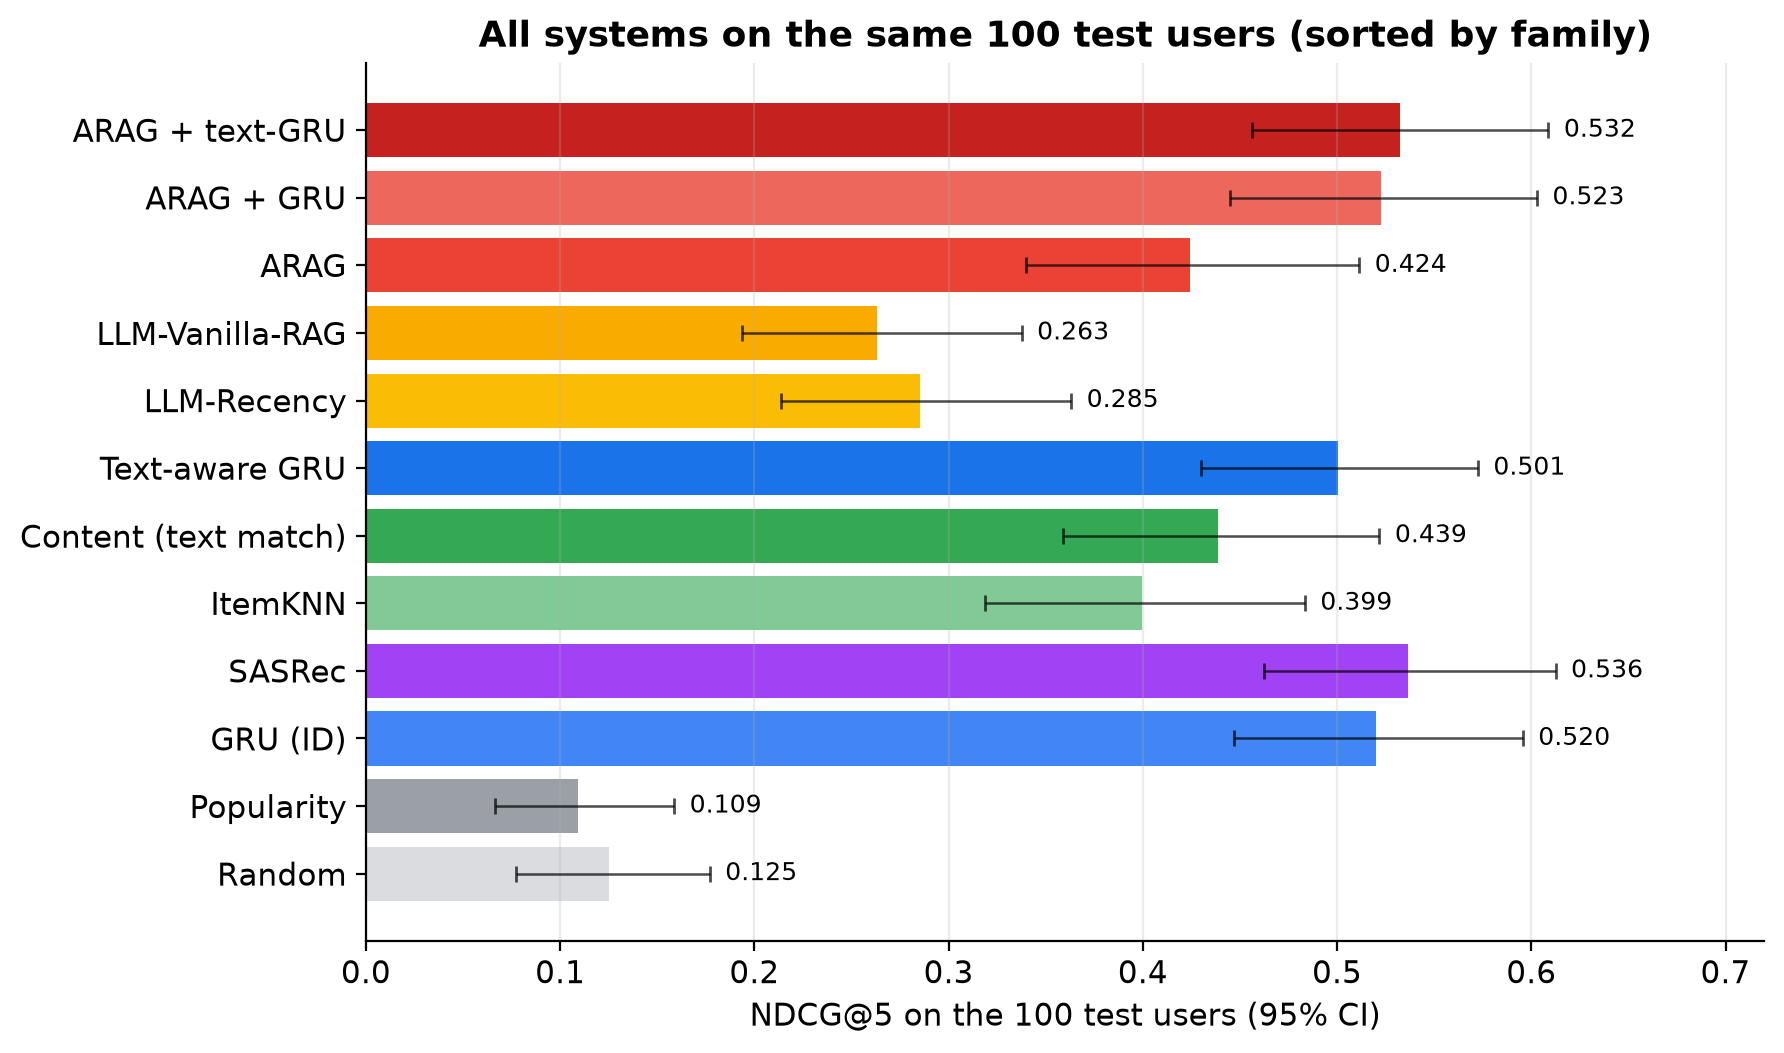
\includegraphics[width=0.85\linewidth]{fig13_sasrec_baseline.png}
  \caption{All systems on the 100 test users (seeded models averaged over three seeds), with
  95\% bootstrap confidence intervals.}
  \label{fig:sasrec}
\end{figure}

\begin{figure}[htbp]
  \centering
  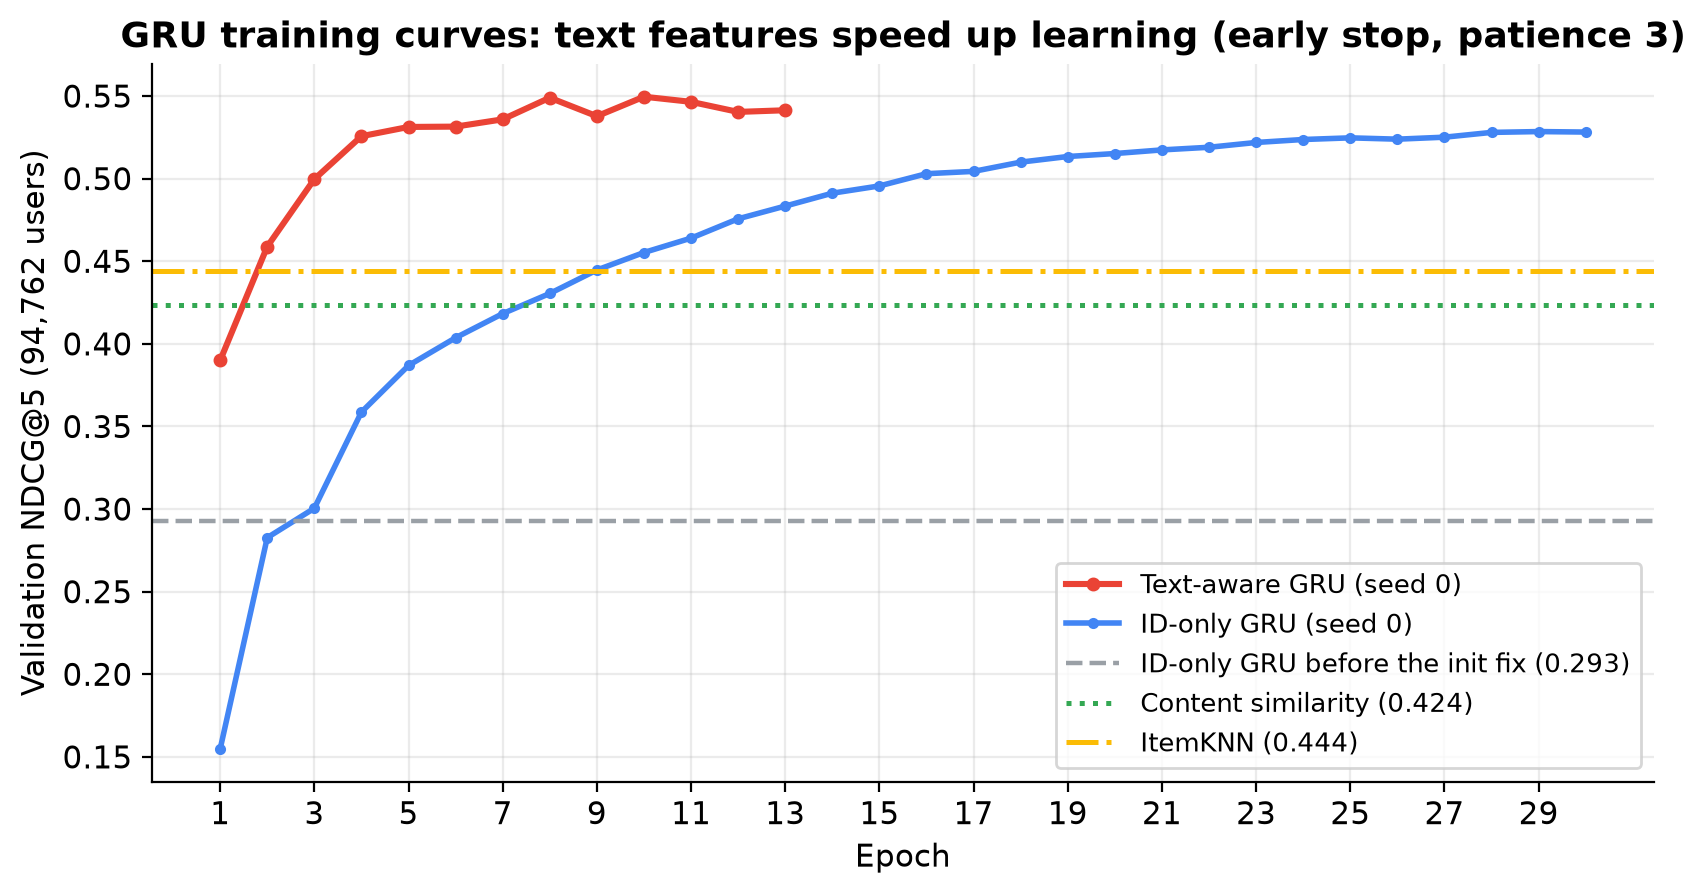
\includegraphics[width=0.75\linewidth]{fig11_text_gru_training.png}
  \caption{Validation NDCG@5 per epoch (seed 0) of the text-aware and ID-only GRUs, against the
  ID-only GRU before the initialisation fix and the two non-learned baselines.}
  \label{fig:textcurve}
\end{figure}

\begin{figure}[htbp]
  \centering
  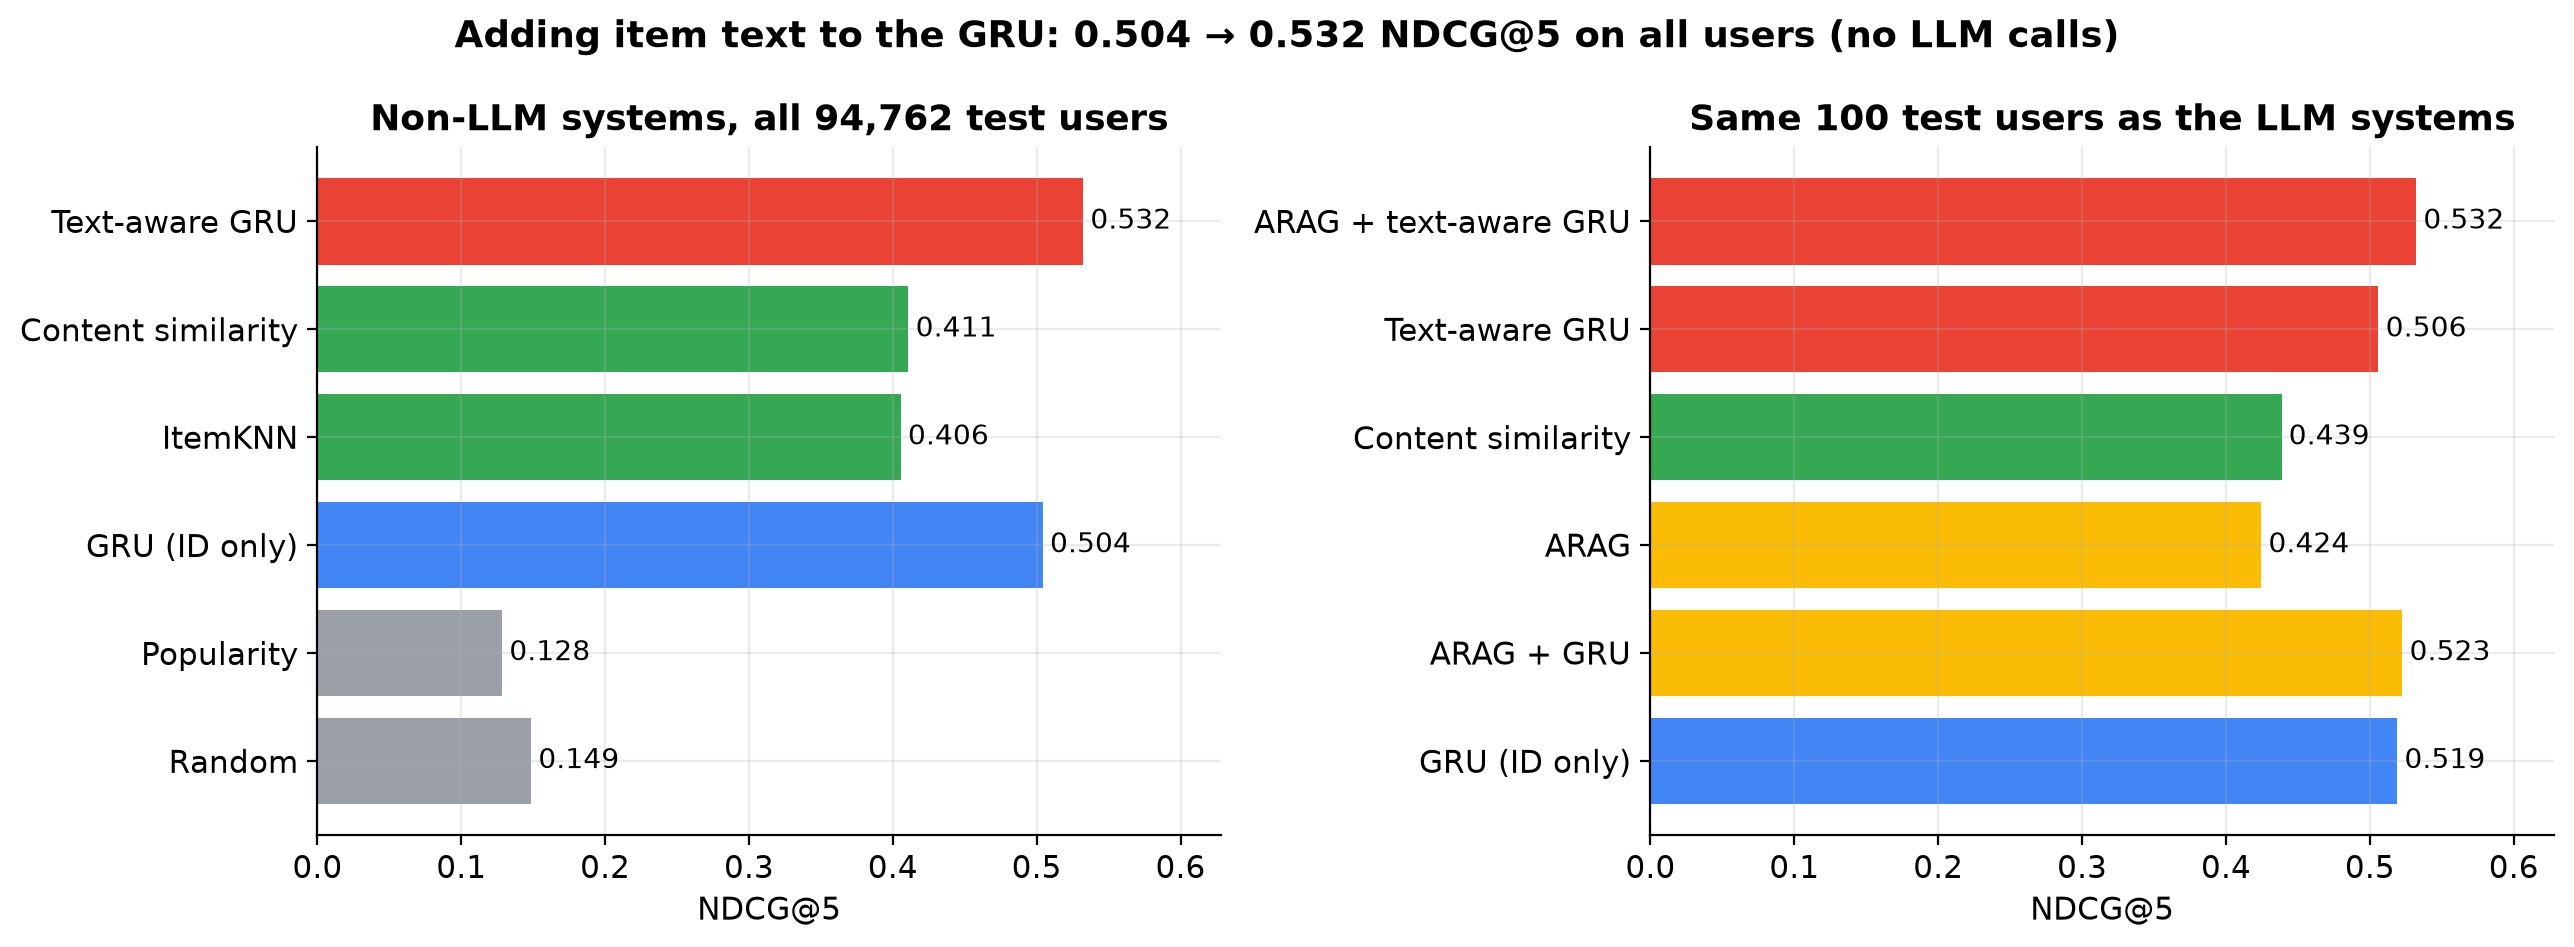
\includegraphics[width=\linewidth]{fig10_content_aware.png}
  \caption{Left: non-LLM systems on all 94{,}762 test users. Right: the same 100 users used for
  the LLM systems.}
  \label{fig:ext}
\end{figure}

\subsection{History length}
\label{sec:history}

\Cref{tab:history} splits all test users by the number of interactions before the test item. The
trained models are nearly flat (GRU $0.497$ for four items, $0.519$ for eleven or more); the
text-aware GRU leads the ID-only GRU in every bucket by $0.024$--$0.027$ (all significant).
Content similarity degrades with longer histories, whose averaged profile becomes less specific,
while ItemKNN improves. On the 100 LLM users (44/30/26 users per bucket, \cref{fig:history}) ARAG
is below the GRU in every bucket, none significantly.

\begin{table}[htbp]
\centering
\caption{NDCG@5 by history length, all test users (seeded models averaged over three seeds).}
\label{tab:history}
\small
\begin{tabular}{lrccccc}
\toprule
History & Users & Content similarity & ItemKNN & GRU (ID only) & Text-aware GRU & SASRec \\
\midrule
4 items & 30{,}451 & 0.420 & 0.389 & 0.497 & 0.521 & 0.502 \\
5--6 & 29{,}707 & 0.417 & 0.398 & 0.503 & 0.530 & 0.508 \\
7--10 & 20{,}678 & 0.402 & 0.419 & 0.510 & 0.536 & 0.511 \\
11+ & 13{,}926 & 0.391 & 0.437 & 0.519 & 0.543 & 0.513 \\
\bottomrule
\end{tabular}

\end{table}

\begin{figure}[htbp]
  \centering
  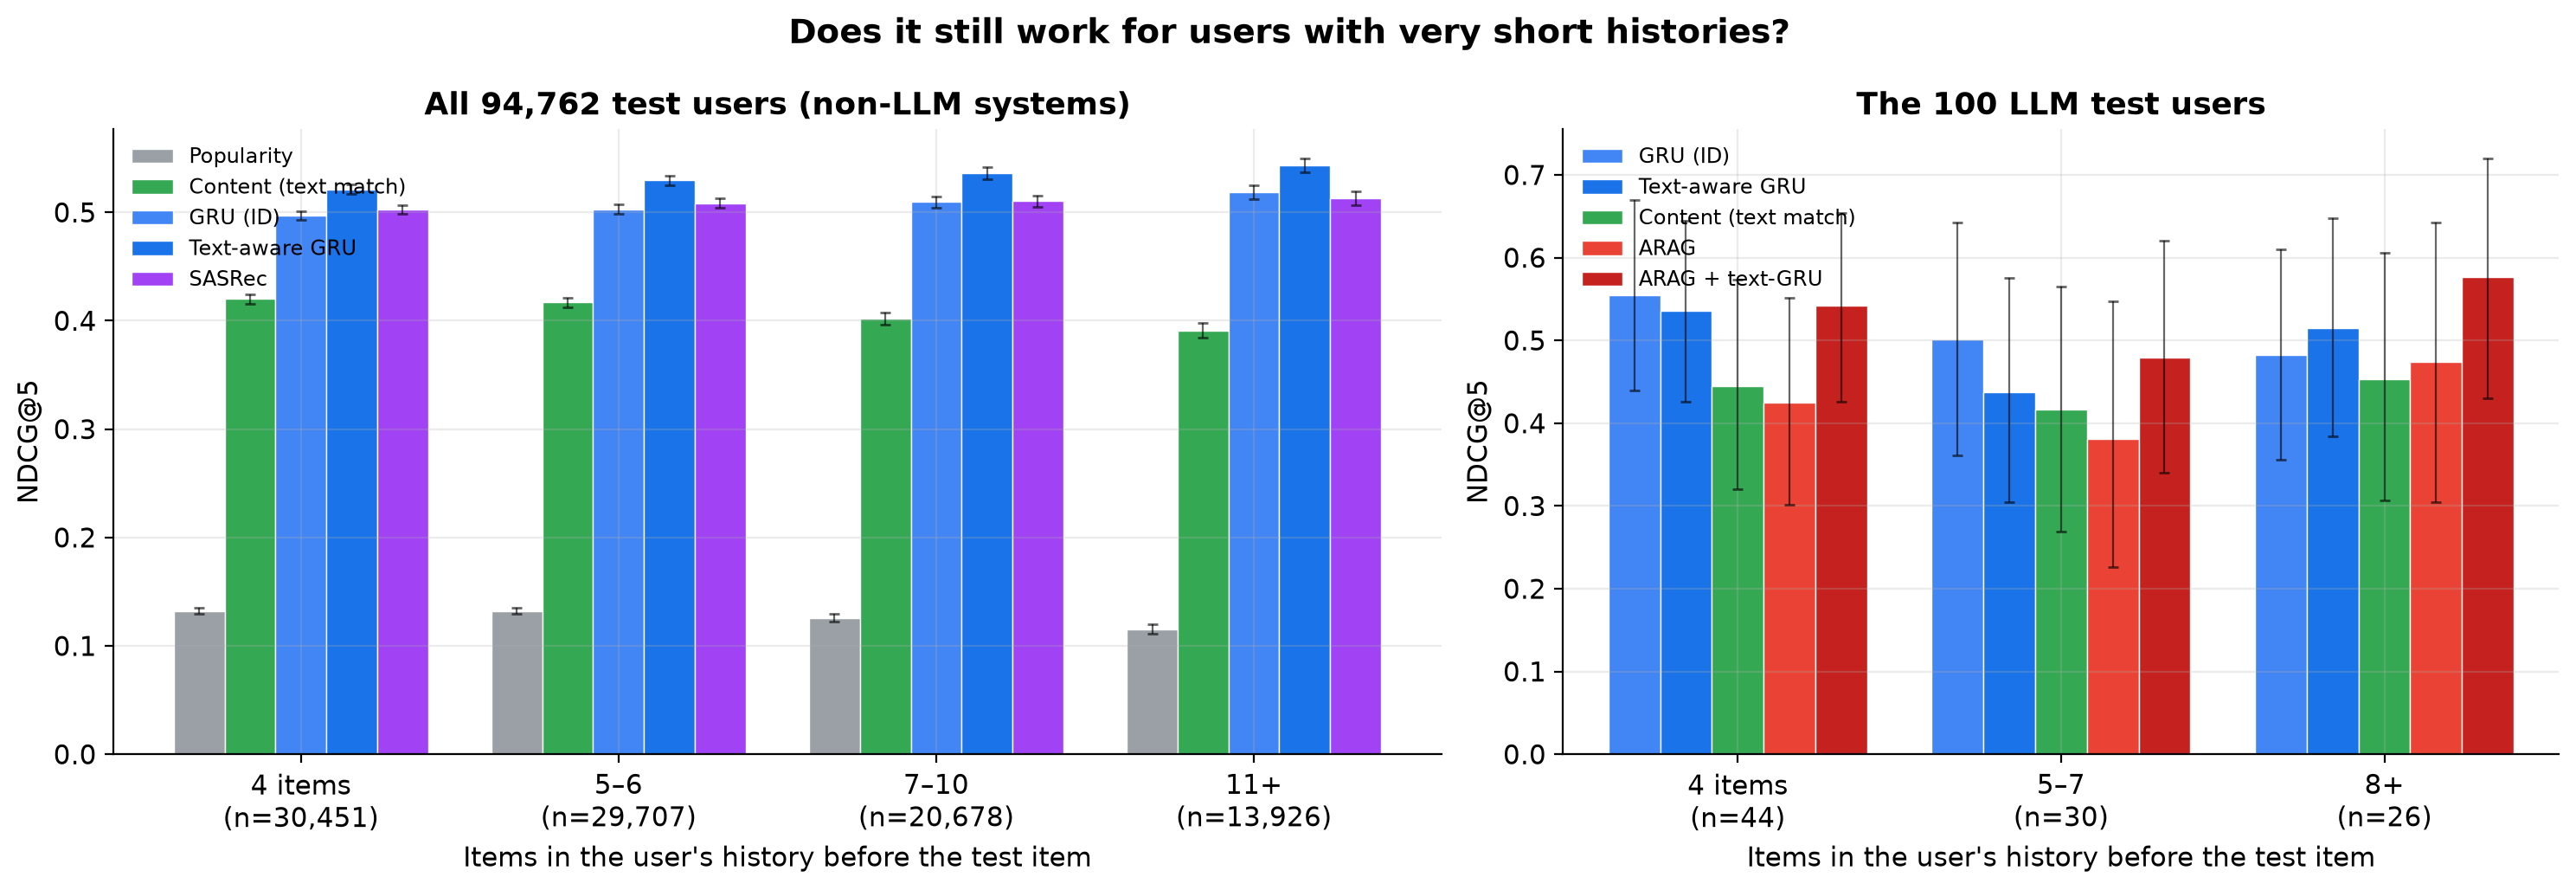
\includegraphics[width=\linewidth]{fig12_history_length_performance.png}
  \caption{NDCG@5 by history length. Left: all test users. Right: the 100 LLM users.}
  \label{fig:history}
\end{figure}

\subsection{Beyond accuracy}

\Cref{tab:beyond} reports, on the 100 users, the popularity lift of each system's top five (mean
$\log(1+\text{train count})$ of the top five minus the 20-candidate average), intra-list
diversity (one minus the mean pairwise MiniLM cosine of the top five) and coverage (distinct top-5
items over distinct candidates). ARAG's lift is $0.127$, against $0.74$--$0.79$ for the trained
models and $0.98$ for ItemKNN, and its coverage is the highest of the learned systems ($0.275$ vs.\
$\approx0.25$). Diversity is essentially equal ($\approx0.72$) except for content similarity
($0.646$). Fusion at the chosen $\alpha$ inherits the trained model's popularity bias.

\begin{table}[htbp]
\centering
\caption{Beyond-accuracy metrics on the 100 test users (seeded models averaged over three seeds).}
\label{tab:beyond}
\small
\begin{tabular}{lcccc}
\toprule
System & NDCG@5 & Popularity lift & Diversity (ILD) & Coverage \\
\midrule
Popularity & 0.109 & 1.783 & 0.723 & 0.181 \\
ItemKNN & 0.399 & 0.983 & 0.723 & 0.241 \\
Content similarity & 0.439 & 0.083 & 0.646 & 0.278 \\
GRU (ID only) & 0.520 & 0.768 & 0.721 & 0.252 \\
Text-aware GRU & 0.501 & 0.741 & 0.718 & 0.253 \\
SASRec & 0.536 & 0.787 & 0.718 & 0.247 \\
LLM-Recency & 0.285 & 0.162 & 0.724 & 0.281 \\
LLM-Vanilla-RAG & 0.263 & 0.278 & 0.725 & 0.273 \\
ARAG & 0.424 & 0.127 & 0.726 & 0.275 \\
ARAG + GRU & 0.523 & 0.728 & 0.720 & 0.254 \\
ARAG + text-GRU & 0.532 & 0.750 & 0.717 & 0.254 \\
\bottomrule
\end{tabular}

\end{table}

\begin{figure}[htbp]
  \centering
  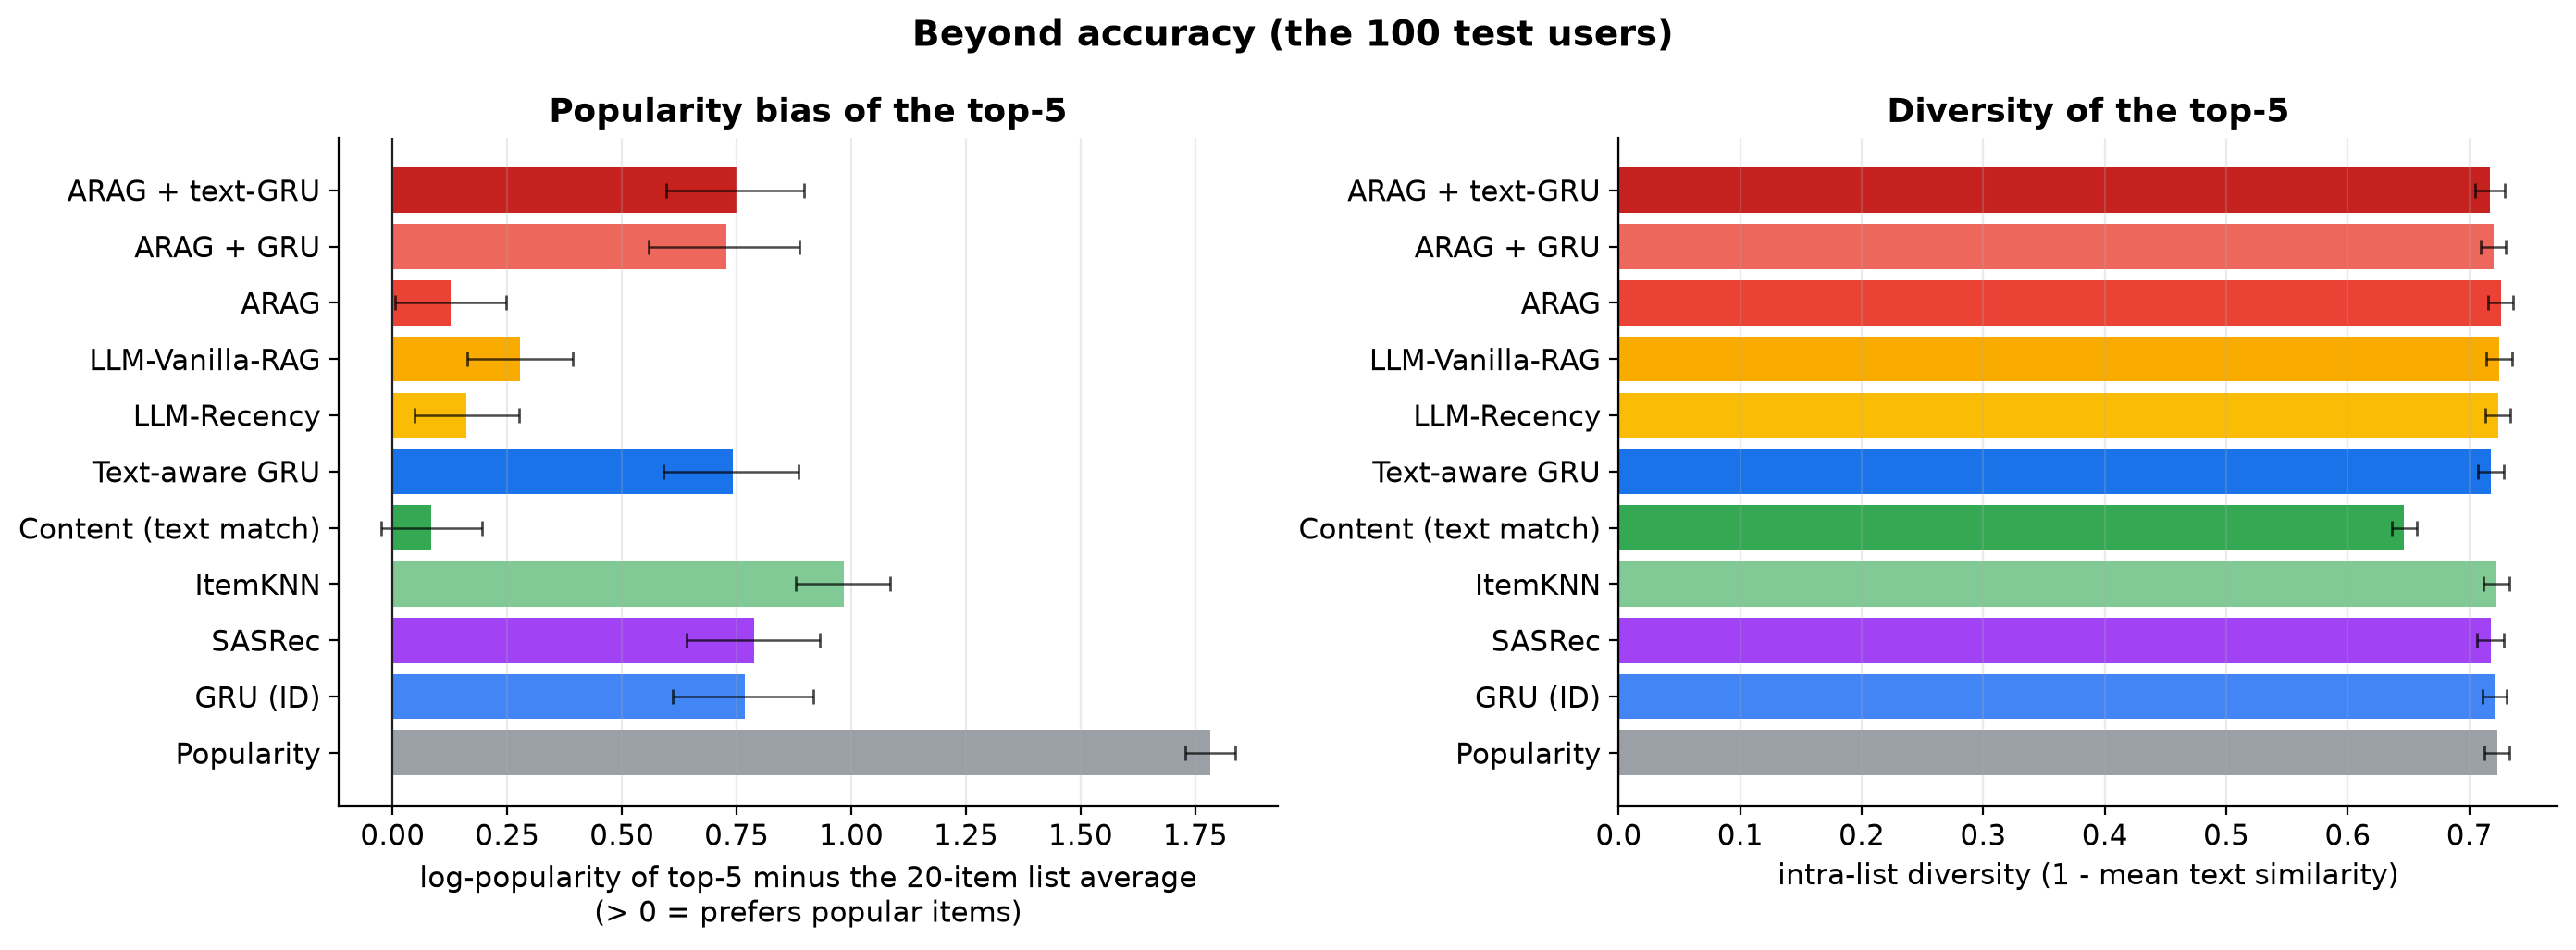
\includegraphics[width=\linewidth]{fig14_beyond_accuracy.png}
  \caption{Popularity bias (left) and diversity (right) of each system's top five.}
  \label{fig:beyond}
\end{figure}

% ================================================================ 8 discussion
\section{Discussion}
\label{sec:discussion}

\subsection{What the base paper did and did not show}

ARAG's claims are about LLM-based recommenders, and they hold: the agentic decomposition beats
single-prompt baselines and its NLI+CSA components contribute. The paper does not report trained
sequential baselines, and on our protocol those are more accurate than ARAG. Our results therefore
do not contradict the paper; they show that its comparison was incomplete. They are also limited
to one category, one LLM and 100 LLM-evaluated users. This pattern --- carefully tuned standard
baselines matching or beating newer methods --- echoes \citet{dacrema2019really}.

\subsection{Why fusion helps ARAG but not the GRU}

The two rankers make different mistakes: ARAG judges candidates by their descriptions against a
language summary of the user, the GRU by co-occurrence patterns across 625k interactions. Adding a
small amount of ARAG's ranking to the GRU ($\alpha^*=0.2$) recovers most of the GRU's accuracy and
substantially improves ARAG, but the extra information is not enough to lift the fused system above
the GRU at $n=100$. Content similarity is statistically tied with ARAG, which suggests that much of
ARAG's skill on this task comes from reading item text.

\subsection{What text adds to a sequence model}
\label{sec:disc-representation}

The text-aware GRU changes only the item vector (\cref{eq:textgru}). Its gain over the correctly
trained ID-only GRU is modest ($+0.026$) but consistent across seeds and history lengths, and it
learns much faster (\cref{fig:textcurve}). Text features place rarely seen items near semantically
similar ones, in line with transferable text-based sequence models \citep{hou2022unisrec}. An
earlier version of this report attributed a far larger gain ($+0.17$) to text; that figure was an
artefact of the initialisation bug (\cref{app:initbug}).

\subsection{Why keep an LLM?}

ARAG has the lowest popularity bias of any learned system and the highest coverage, produces
natural-language explanations for every recommendation, and handles free-text queries (used by our
demonstrator's search). These properties are not measured by NDCG@5 but matter in a product.

\subsection{Cost--quality trade-off}

ARAG needs seven LLM calls per user (about \$1 per 100-user evaluation with
\texttt{gpt-4o-mini}, and seconds of latency per user). The text-aware GRU scores all 94{,}762 test
users in seconds on a CPU at no marginal cost. On this protocol the trained models are the better
operating point for accuracy; ARAG is the better operating point for explanation and low
popularity bias.

\subsection{A methodological lesson: candidate construction can manufacture conclusions}

An earlier version of the study sampled negatives uniformly from all 137{,}260 catalogue items
with text. Because 81\% of those items have no interactions, a mean of 15.5 of the 19 negatives
were unknown to popularity (all tied at zero) and to the GRU (all mapped to one OOV embedding).
The effective task for those systems was a choice among about 4.5 items. Popularity reached
Hit@5 $=0.97$, the GRU NDCG@5 $=0.82$, and fusion appeared to improve ARAG by $+0.349$
(``H1 supported''). The flaw was found in review; the lists were rebuilt with
popularity-matched in-vocabulary negatives, every system was re-evaluated and the GRU retrained.
The conclusion reversed (\cref{fig:flaw}). The general point, also made by
\citet{krichene2020sampled}, is that sampled-candidate protocols must be checked for shortcuts
that some systems can exploit and others cannot. A second error --- the GRU's embedding
initialisation (\cref{app:initbug}) --- reversed the conclusion again; it was exposed only when an
independent architecture (SASRec) showed the same symptom. A weak baseline should be a reason to
check the baseline.

\begin{figure}[htbp]
  \centering
  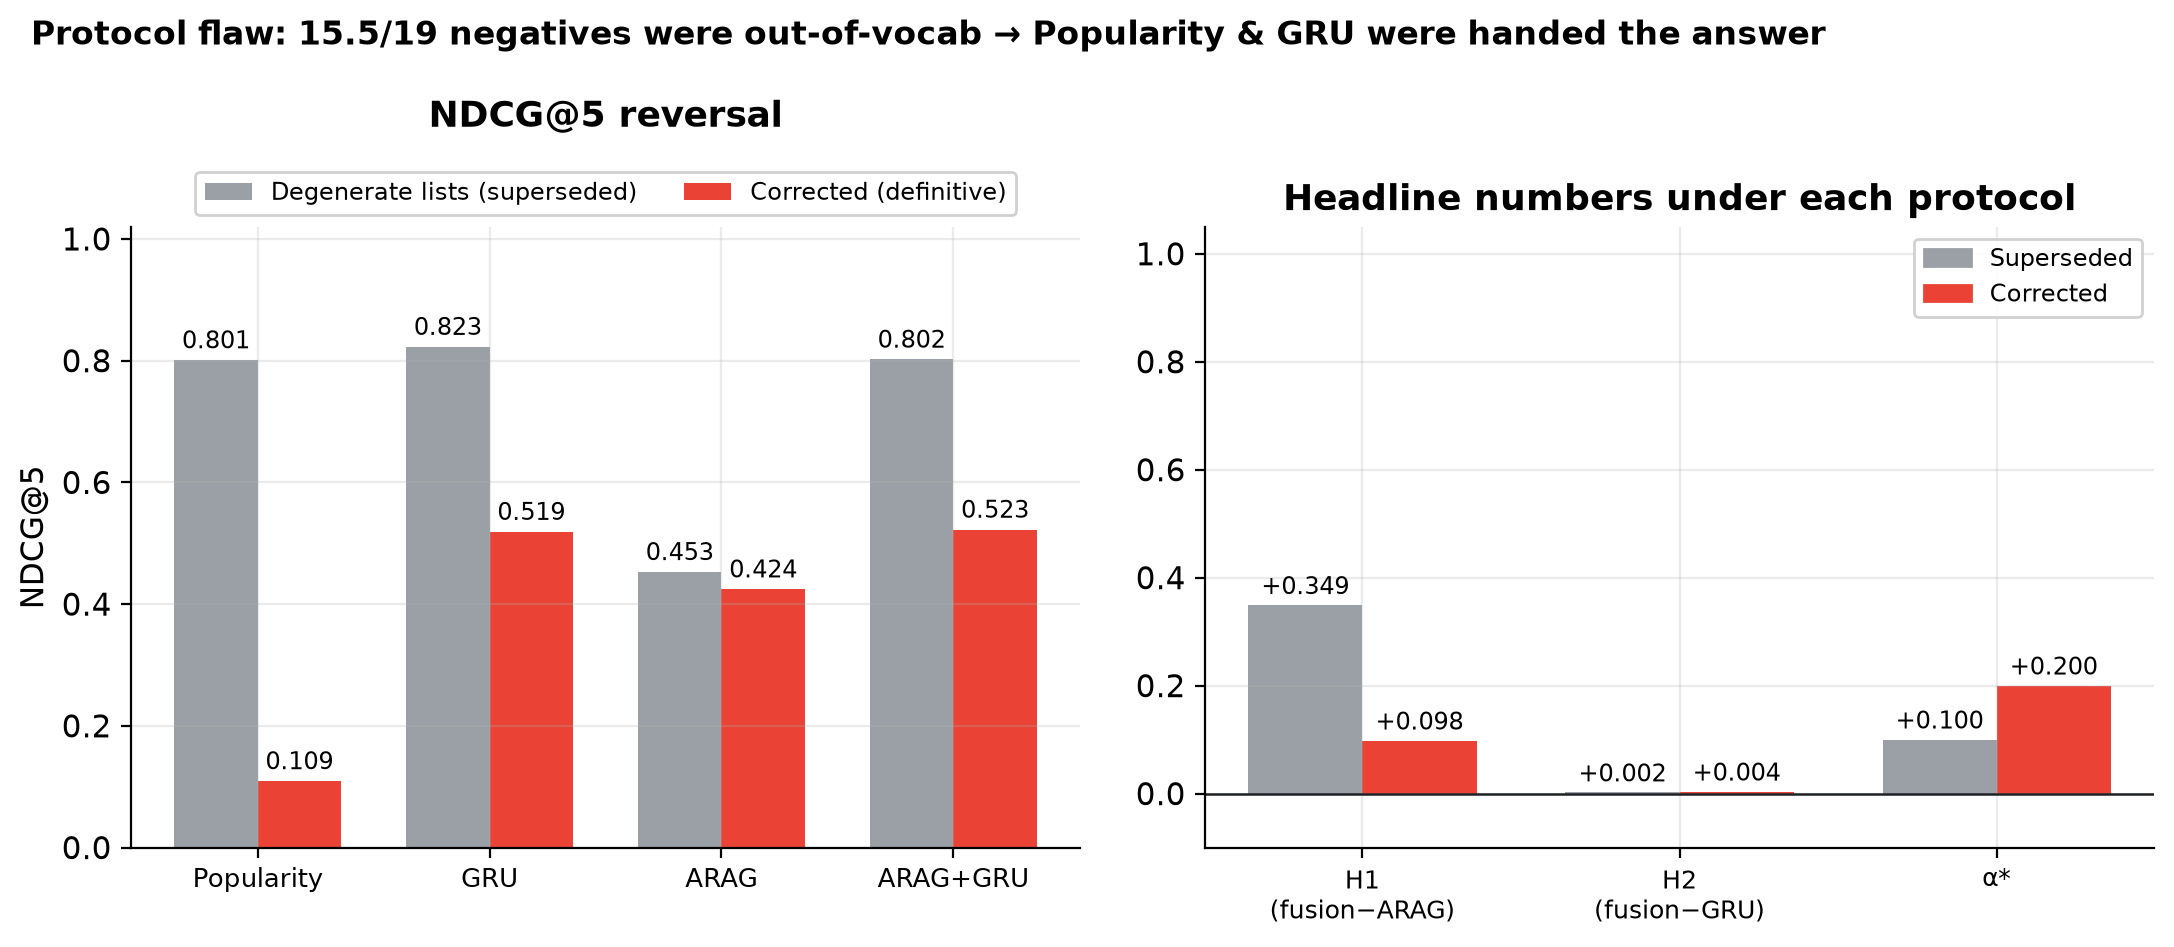
\includegraphics[width=0.85\linewidth]{fig07_protocol_flaw.png}
  \caption{The original (degenerate) candidate lists versus the corrected lists (right panel:
  final numbers with the corrected GRU).}
  \label{fig:flaw}
\end{figure}

% ================================================================ 9 threats
\section{Threats to Validity}
\label{sec:threats}

\begin{enumerate}
  \item \textbf{Sample size.} Only 100 users are evaluated with the LLM (cost). Confidence intervals
  on NDCG@5 differences are roughly $\pm0.08$--$0.10$, so the top systems (GRU, SASRec,
  text-aware GRU and the fusions) cannot be separated from each other, and ARAG versus the GRU is
  borderline. About 300 users ($\approx\$3$)
  would be needed to resolve differences of $\sim0.05$.
  \item \textbf{Sampled negatives.} Popularity-matched negatives remove the popularity shortcut but
  are easier than candidates mined by a real retriever. Results describe ranking quality on hard
  20-item lists, not end-to-end retrieval quality.
  \item \textbf{Slight tilt of the negatives.} Popularity scores slightly below random (Hit@5 0.213
  vs.\ 0.252 on all users), so negatives are on average a little more popular than targets. This
  slightly disadvantages frequency-sensitive models, including the GRUs. The effect ($\sim0.04$
  Hit@5) is much smaller than the gaps we interpret.
  \item \textbf{Leave-last-out leakage.} Other users' later interactions can appear in the training
  data of the GRUs and ItemKNN. This is inherent to the official split and affects those systems
  equally; content similarity does not use other users' data.
  \item \textbf{Training budget and search.} The ID-only GRU was still improving slowly at the
  30-epoch cap and the hyperparameter grids are small; the trained models are, if anything,
  under-estimated.
  \item \textbf{Tuning noise.} $\alpha$ and $\theta$ are tuned on 100 validation users; the
  validation and test $\alpha$ curves differ in detail near their maxima ($\alpha=0.1$--$0.3$).
  \item \textbf{Scope.} One category, one dataset, one LLM. The study is ARAG-inspired, not an
  exact reproduction: the paper does not publish prompts, its threshold or its candidate
  construction, and it used \texttt{gpt-3.5-turbo} on the 2016 Amazon data.
  \item \textbf{Offline metrics only.} No online or human evaluation; one held-out item per user
  defines relevance.
\end{enumerate}

% ================================================================ 10 conclusion
\section{Conclusion and Future Work}
\label{sec:conclusion}

We built an ARAG-style agentic recommender and evaluated it against, and fused with, trained
sequential models under a protocol that isolates ranking and tests every contrast statistically.
First, the agentic pipeline significantly beats simpler LLM baselines and its NLI+CSA ablation,
reproducing the base paper's claims on a new category and model. Second, properly trained
sequential recommenders --- GRU4Rec, SASRec and our text-aware GRU --- are more accurate than ARAG
(NDCG@5 $0.505$--$0.530$ on all test users; ARAG $0.424$ on its 100 users, significantly below
SASRec), at no per-request cost. Fusing the GRU into ARAG significantly improves ARAG (H1) but not
the GRU (H2). Third, ARAG's distinctive value lies beyond accuracy: much lower popularity bias,
higher coverage and natural-language explanations. Finally, both a candidate-construction flaw
and an initialisation bug reversed our headline conclusion before they were found; evaluation
pipelines and baselines must be audited, not just the proposed method.

Future work: a larger LLM-evaluated sample to separate the top systems; negatives mined by a
retriever; SASRec with the text-aware item representation; review text as an item feature; feeding
the trained model's scores to the IRA agent as an explicit feature instead of fusing afterwards;
and replication on further categories and LLMs.

% ================================================================ references
\bibliographystyle{plainnat}
\begin{thebibliography}{99}

\bibitem[Cho et~al.(2014)]{cho2014learning}
K.~Cho, B.~van Merri{\"e}nboer, C.~Gulcehre, D.~Bahdanau, F.~Bougares, H.~Schwenk, and Y.~Bengio.
\newblock Learning phrase representations using {RNN} encoder--decoder for statistical machine translation.
\newblock In \emph{Proceedings of EMNLP}, 2014.

\bibitem[Dacrema et~al.(2019)]{dacrema2019really}
M.~Ferrari Dacrema, P.~Cremonesi, and D.~Jannach.
\newblock Are we really making much progress? {A} worrying analysis of recent neural recommendation approaches.
\newblock In \emph{Proceedings of ACM RecSys}, 2019.

\bibitem[Efron and Tibshirani(1993)]{efron1993bootstrap}
B.~Efron and R.~J. Tibshirani.
\newblock \emph{An Introduction to the Bootstrap}.
\newblock Chapman \& Hall, 1993.

\bibitem[Hidasi et~al.(2016)]{hidasi2016session}
B.~Hidasi, A.~Karatzoglou, L.~Baltrunas, and D.~Tikk.
\newblock Session-based recommendations with recurrent neural networks.
\newblock In \emph{International Conference on Learning Representations (ICLR)}, 2016.

\bibitem[Hou et~al.(2022)]{hou2022unisrec}
Y.~Hou, S.~Mu, W.~X. Zhao, Y.~Li, B.~Ding, and J.-R. Wen.
\newblock Towards universal sequence representation learning for recommender systems.
\newblock In \emph{Proceedings of ACM SIGKDD}, 2022.

\bibitem[Hou et~al.(2024a)]{hou2024bridging}
Y.~Hou, J.~Li, Z.~He, A.~Yan, X.~Chen, and J.~McAuley.
\newblock Bridging language and items for retrieval and recommendation.
\newblock \emph{arXiv preprint arXiv:2403.03952}, 2024.

\bibitem[Hou et~al.(2024b)]{hou2024llmrank}
Y.~Hou, J.~Zhang, Z.~Lin, H.~Lu, R.~Xie, J.~McAuley, and W.~X. Zhao.
\newblock Large language models are zero-shot rankers for recommender systems.
\newblock In \emph{Proceedings of ECIR}, 2024.

\bibitem[J{\"a}rvelin and Kek{\"a}l{\"a}inen(2002)]{jarvelin2002cumulated}
K.~J{\"a}rvelin and J.~Kek{\"a}l{\"a}inen.
\newblock Cumulated gain-based evaluation of {IR} techniques.
\newblock \emph{ACM Transactions on Information Systems}, 20(4):422--446, 2002.

\bibitem[Johnson et~al.(2019)]{johnson2019billion}
J.~Johnson, M.~Douze, and H.~J{\'e}gou.
\newblock Billion-scale similarity search with {GPU}s.
\newblock \emph{IEEE Transactions on Big Data}, 7(3):535--547, 2019.

\bibitem[Kang and McAuley(2018)]{kang2018self}
W.-C. Kang and J.~McAuley.
\newblock Self-attentive sequential recommendation.
\newblock In \emph{Proceedings of IEEE ICDM}, 2018.

\bibitem[Krichene and Rendle(2020)]{krichene2020sampled}
W.~Krichene and S.~Rendle.
\newblock On sampled metrics for item recommendation.
\newblock In \emph{Proceedings of ACM SIGKDD}, 2020.

\bibitem[Maragheh et~al.(2025)]{maragheh2025arag}
R.~Y. Maragheh, P.~Vadla, P.~Gupta, K.~Zhao, A.~Inan, K.~Yao, J.~Xu, P.~Kanumala, J.~Cho, and S.~Kumar.
\newblock {ARAG}: Agentic retrieval augmented generation for personalized recommendation.
\newblock \emph{arXiv preprint arXiv:2506.21931}, 2025.

\bibitem[Reimers and Gurevych(2019)]{reimers2019sentence}
N.~Reimers and I.~Gurevych.
\newblock Sentence-{BERT}: Sentence embeddings using {S}iamese {BERT}-networks.
\newblock In \emph{Proceedings of EMNLP-IJCNLP}, 2019.

\bibitem[Sarwar et~al.(2001)]{sarwar2001item}
B.~Sarwar, G.~Karypis, J.~Konstan, and J.~Riedl.
\newblock Item-based collaborative filtering recommendation algorithms.
\newblock In \emph{Proceedings of WWW}, 2001.

\bibitem[Wang et~al.(2020)]{wang2020minilm}
W.~Wang, F.~Wei, L.~Dong, H.~Bao, N.~Yang, and M.~Zhou.
\newblock {MiniLM}: Deep self-attention distillation for task-agnostic compression of pre-trained transformers.
\newblock In \emph{Advances in Neural Information Processing Systems (NeurIPS)}, 2020.

\end{thebibliography}

% ================================================================ appendices
\appendix

\section{Worked Example}
\label{app:example}

A real test user (\texttt{AEDTQXNMWBEI7UECETV5JVUEWNDQ}) with a four-item history: \textit{The
Legend of Zelda: Breath of the Wild} (Wii U), \textit{Need for Speed Most Wanted U} (Wii U),
\textit{Hot Wheels World's Best Driver} and \textit{LEGO Marvel} (PC). The frozen list contains
twenty plausible gaming products --- for example \textit{Demon's Souls} (PS3), \textit{New Super
Mario Bros.\ U}, a Luigi amiibo, \textit{Ghost of Tsushima} (PS4), PS4 controller accessories and
two gaming headsets. The held-out target is an \textit{ARKARTECH Gaming Headset}. Every
negative is a known, reviewed product, illustrating that the corrected lists contain no trivial
zero-interaction decoys: a ranker must infer from four console-game reviews that an accessory
such as a headset is a plausible next item.

\section{Errata: the Superseded Run}
\label{app:errata}

\begin{table}[h]
\centering
\caption{Original (degenerate lists) versus corrected-list results, both with the GRU before
the initialisation fix (\cref{app:initbug}).}
\label{tab:errata}
\small
\begin{tabular}{lcc}
\toprule
Quantity & Original lists & Corrected lists \\
\midrule
Unknown negatives per list (of 19) & 15.5 & 0 \\
Popularity NDCG@5 & 0.801 & 0.109 \\
GRU NDCG@5 (all users) & 0.823 & 0.279 \\
ARAG NDCG@5 & 0.453 & 0.424 \\
$\alpha^*$ & 0.1 & 0.9 \\
H1 (ARAG + GRU $-$ ARAG) & $+0.349$ ``significant'' & $-0.013$ n.s. \\
H2 (ARAG + GRU $-$ GRU) & $+0.002$ n.s. & $+0.174$ significant \\
ARAG vs.\ Recency / Vanilla-RAG & n.s. & both significant \\
\bottomrule
\end{tabular}
\end{table}

\section{Errata: the GRU Initialisation Bug}
\label{app:initbug}

The first version of this report used PyTorch's default $\mathcal{N}(0,1)$ initialisation for
the GRU's item embeddings. With tied input and output embeddings, the initial logits are dot
products of two such vectors, the softmax over 25{,}527 items is saturated (initial loss $\approx30$
versus $\ln 25{,}527\approx10$) and training stalls. The GRU reached only $0.293$ validation and
$0.279$ test NDCG@5, which we attributed to short histories. When SASRec showed the same symptom,
we re-initialised both models from $\mathcal{N}(0,0.02^2)$, retrained both GRUs (same grid and
seeds, epoch cap raised from 12 to 30), re-tuned $\alpha$ on validation and replayed the entire
evaluation from the LLM cache at zero cost. The history-length analysis (\cref{sec:history})
independently rules out the short-history explanation.

\begin{table}[h]
\centering
\caption{Results before and after the initialisation fix.}
\label{tab:initbug}
\small
\begin{tabular}{lcc}
\toprule
Quantity & Before fix & After fix \\
\midrule
GRU validation NDCG@5 (seed 0) & 0.293 & 0.528 \\
GRU test NDCG@5, all users & 0.279 & 0.505 \\
Text-aware GRU test NDCG@5, all users & 0.461 & 0.530 \\
GRU NDCG@5, 100 users (seed 0) & 0.238 & 0.519 \\
$\alpha^*$ (ARAG + GRU) & 0.9 & 0.2 \\
H1 (ARAG + GRU $-$ ARAG) & $-0.013$ n.s. & $+0.098$ significant \\
H2 (ARAG + GRU $-$ GRU) & $+0.174$ significant & $+0.004$ n.s. \\
\bottomrule
\end{tabular}
\end{table}

At the same time we corrected the bootstrap for all-users comparisons, which had resampled a
random 20{,}000-user subset (making those intervals about twice too wide and slightly off-centre);
it now draws exact bootstrap means for all 94{,}762 users. No 100-user interval changed.

\section{Reproducibility}
\label{app:repro}

All code, configuration and results are in the project repository. The full pipeline is:
{\small
\begin{verbatim}
make setup                      # environment
make data lists index           # dataset, frozen lists, MiniLM + FAISS
make gru gru-text sasrec        # ID-only GRU, text-aware GRU, SASRec (grid + 3 seeds)
make eval                       # all systems (LLM calls disk-cached)
make report verify              # results/, and re-derive every metric from raw predictions
make extra                      # history length, SASRec contrasts, beyond-accuracy
python scripts/make_figures.py  # figures
python scripts/make_paper_tables.py   # the LaTeX tables of this report
\end{verbatim}
}
A zero-cost replay of the full evaluation is
\texttt{REPLAY\_ONLY=1 OPENAI\_API\_KEY=replay-only-dummy make eval}; any LLM call missing from
the cache raises an error instead of reaching the API. Every table in \cref{sec:results} is
generated from \texttt{results/metrics.json} and \texttt{results/extra\_metrics.json} by
\texttt{scripts/make\_paper\_tables.py}.

\end{document}
